\documentclass[14pt,a4paper]{extarticle}
\usepackage{graphicx}
\usepackage{caption} 
\usepackage{hyperref}
\usepackage[T1]{fontenc}
\usepackage[utf8x]{inputenc}
\usepackage{pdfpages}
\usepackage{libertine}
\usepackage{listings}
\usepackage{xcolor}
\usepackage{enumitem}
\renewcommand{\thesection}{\arabic{section}}
\renewcommand{\familydefault}{\sfdefault}

\definecolor{stringgreen}{RGB}{100, 255, 100}

\lstdefinestyle{fish}{
	basicstyle=\small\ttfamily\color{black},
    keywordstyle=\color{blue},
	stringstyle=\medium\ttfamily\color{green},
    numberstyle=\tiny\color{gray},
    showstringspaces=false,
    tabsize=4,
	frame=single,
    breaklines=true,
    morekeywords={sudo,if,then,else,elif,fi,for,do,done,while,until,in},
}

\lstdefinestyle{json}{
	basicstyle=\small\ttfamily\color{black},
    showstringspaces=false,
    tabsize=2,
    breaklines=true,
}

\lstdefinestyle{sql}{
	basicstyle=\small\ttfamily\color{black},
    keywordstyle=\color{blue},
	stringstyle=\color{stringgreen},
    numberstyle=\tiny\color{gray},
    showstringspaces=false,
    tabsize=4,
    breaklines=true,
	language=SQL
}

\colorlet{punct}{red!60!black}
\definecolor{delim}{RGB}{20,105,176}
\colorlet{numb}{magenta!60!black}

\hypersetup{
    colorlinks=true,
    linkcolor=blue,
    filecolor=blue,      
    urlcolor=blue,
    pdfborder={0 0 0},
    linktocpage      
}

\begin{document}
	\begin{titlepage}
		\centering
		{\scshape\LARGE Big Data \par}
		\vspace{2.5cm}
		{\huge\bfseries ELK Stack Exercise}
		\vfill
		{\normalsize von\par}
		{\normalsize Benjamin Ellmer (\textsc{S2210455012}) \par}
		\vspace{1cm}
		
\includegraphics[width=0.3\textheight]{images/logo.pdf} \par
		\vspace{1cm}
		{\large Mobile Computing Master \par}
		{\large FH Hagenberg \par}
		\vfill
		{\large \today\par}
	\end{titlepage}

	\section*{Step 1}
	\noindent \textbf{Clone repo and run the containers using docker compose:}
	\begin{lstlisting}[style=fish]
git clone https://github.com/Digital-Media/elk-stack-dock
cd elk-stack-dock
docker compose -f docker-compose.yml up -d
	\end{lstlisting}

	\noindent \textbf{Open bash inside logstash container and run simple pipeline:}
	\begin{lstlisting}[style=fish]
docker exec -it elk-stack-dock_logstash_1 /bin/bash
whereis logstash
cd /usr/share/logstash/bin
./logstash -e 'input { stdin { } } output { stdout {} }'
	\end{lstlisting}
	\noindent \textbf{The pipeline fails because data is already in use} \\
	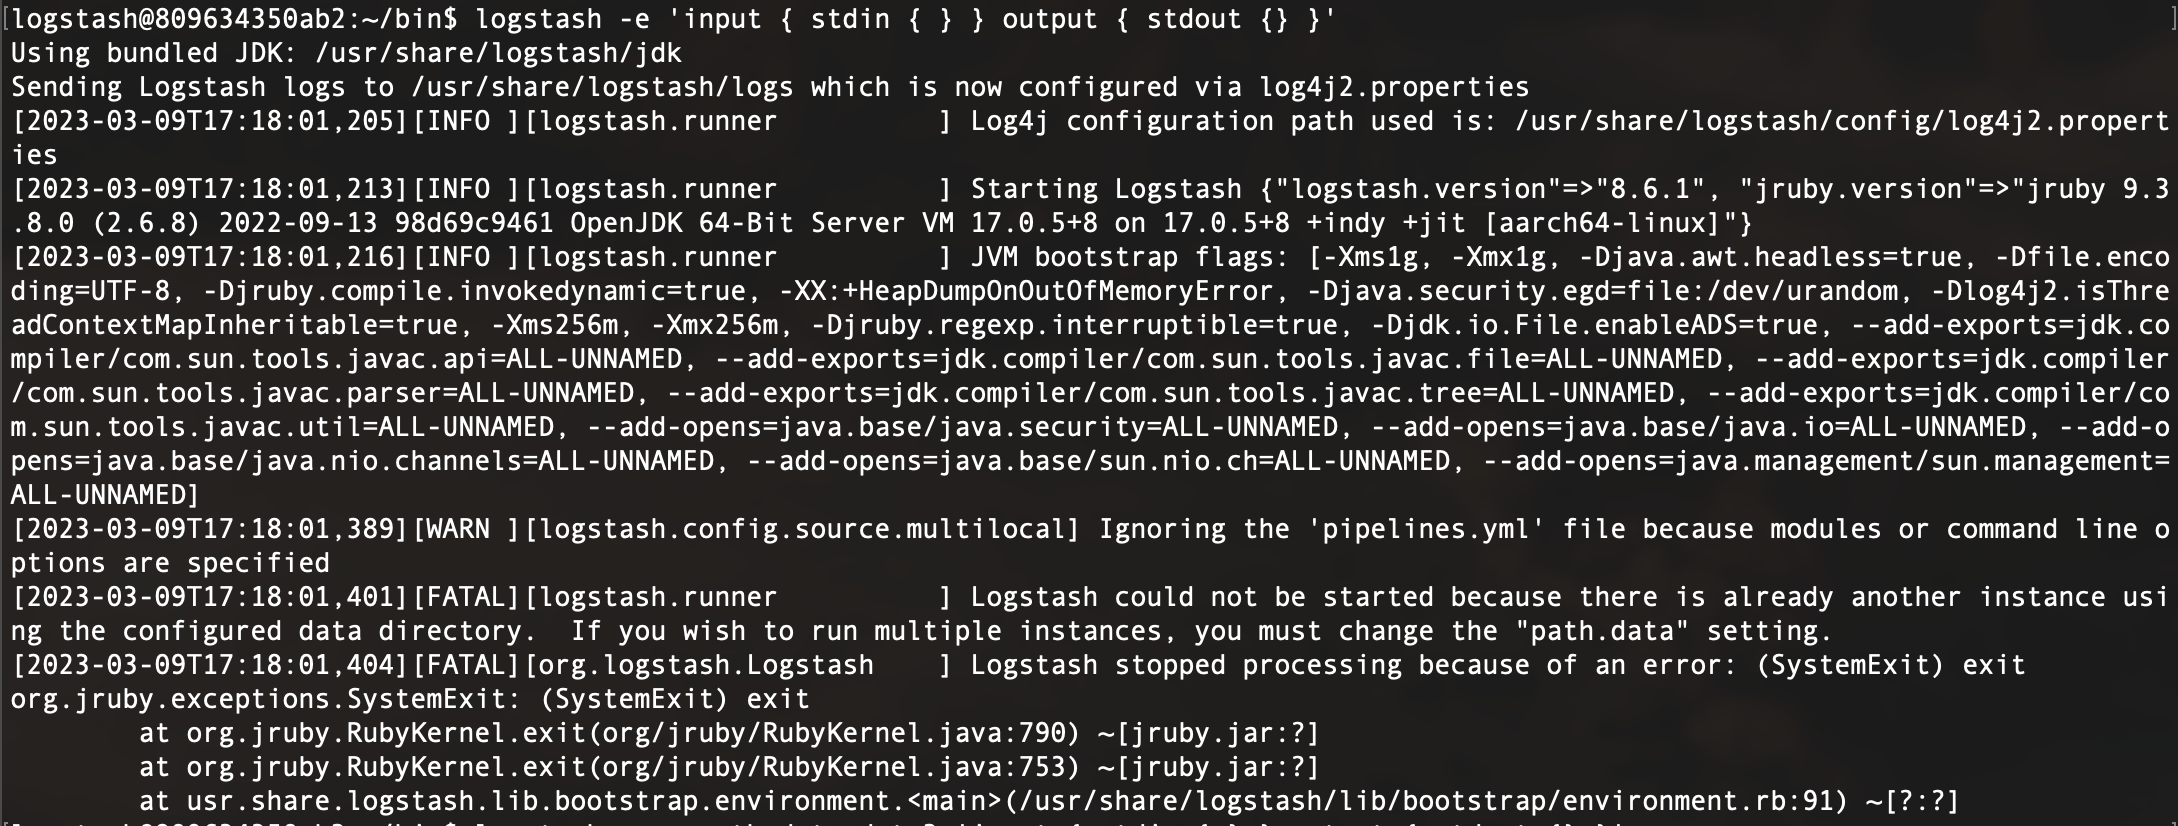
\includegraphics[width=\textwidth]{images/sc01.png} 

	\noindent \textbf{Rerun pipeline using the data2 directory}
	\begin{lstlisting}[style=fish]
logstash --path.data data2 -e 'input { stdin { } } output { stdout {} }'
	\end{lstlisting}
	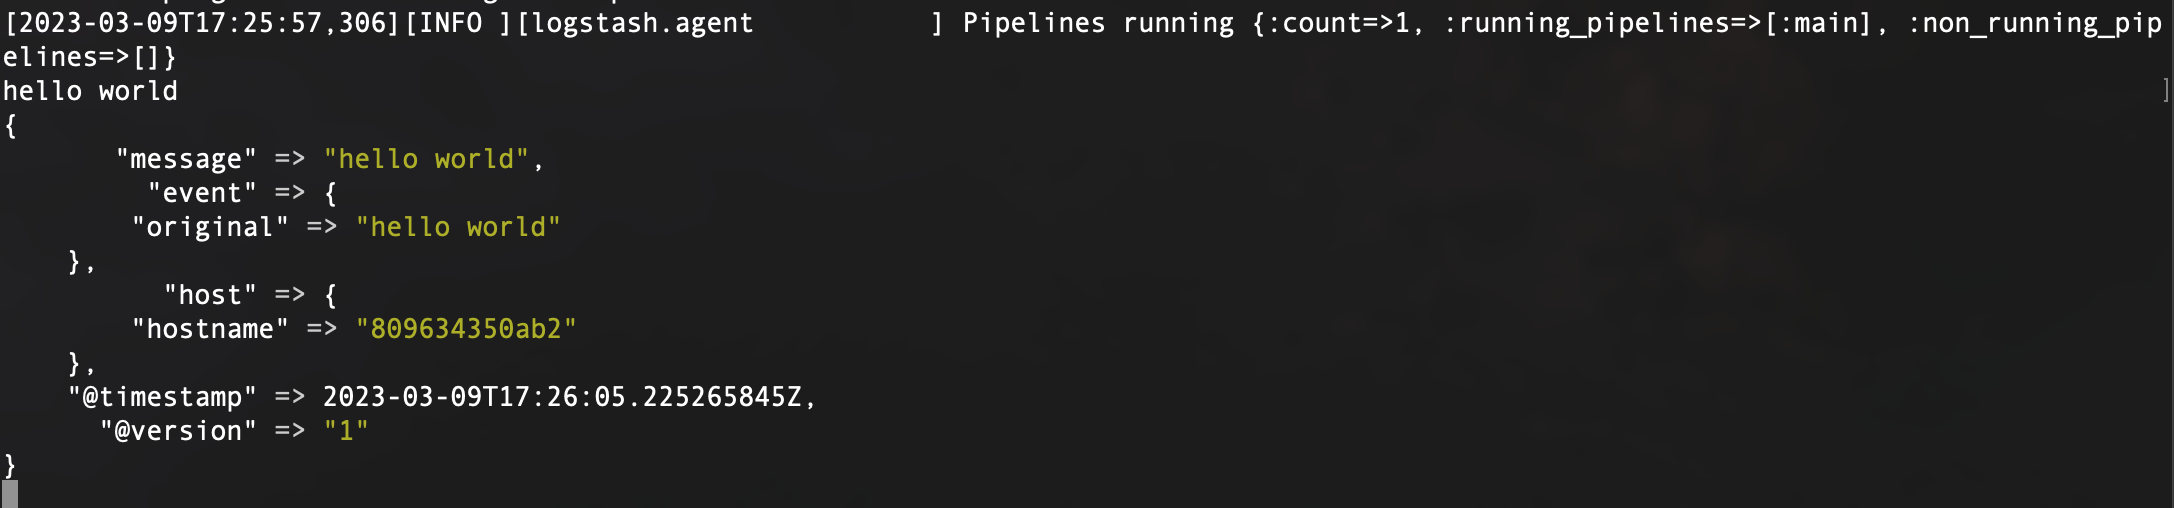
\includegraphics[width=\textwidth]{images/sc02.png} 
	\newpage

	\noindent \textbf{Check if jdbc is installed} 
	\begin{lstlisting}[style=fish]
logstash-plugin list --verbose | grep "jdbc"
	\end{lstlisting}
	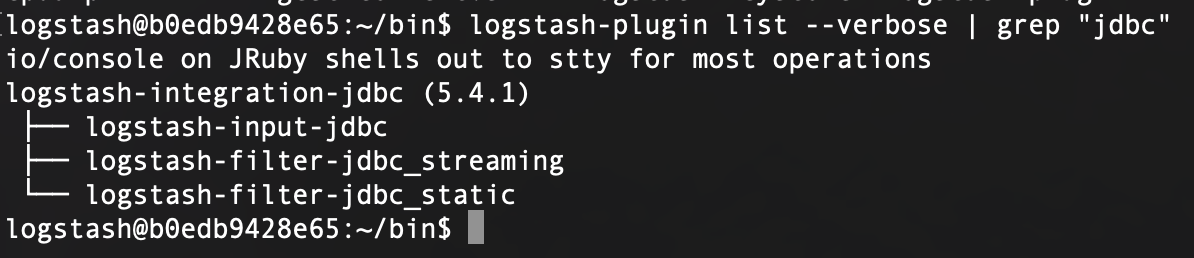
\includegraphics[width=\textwidth]{images/sc03.png} 

	\noindent \textbf{Check pipeline configuration} 
	\begin{lstlisting}[style=fish]
logstash --path.settings /usr/share/logstash/config -t
	\end{lstlisting}
	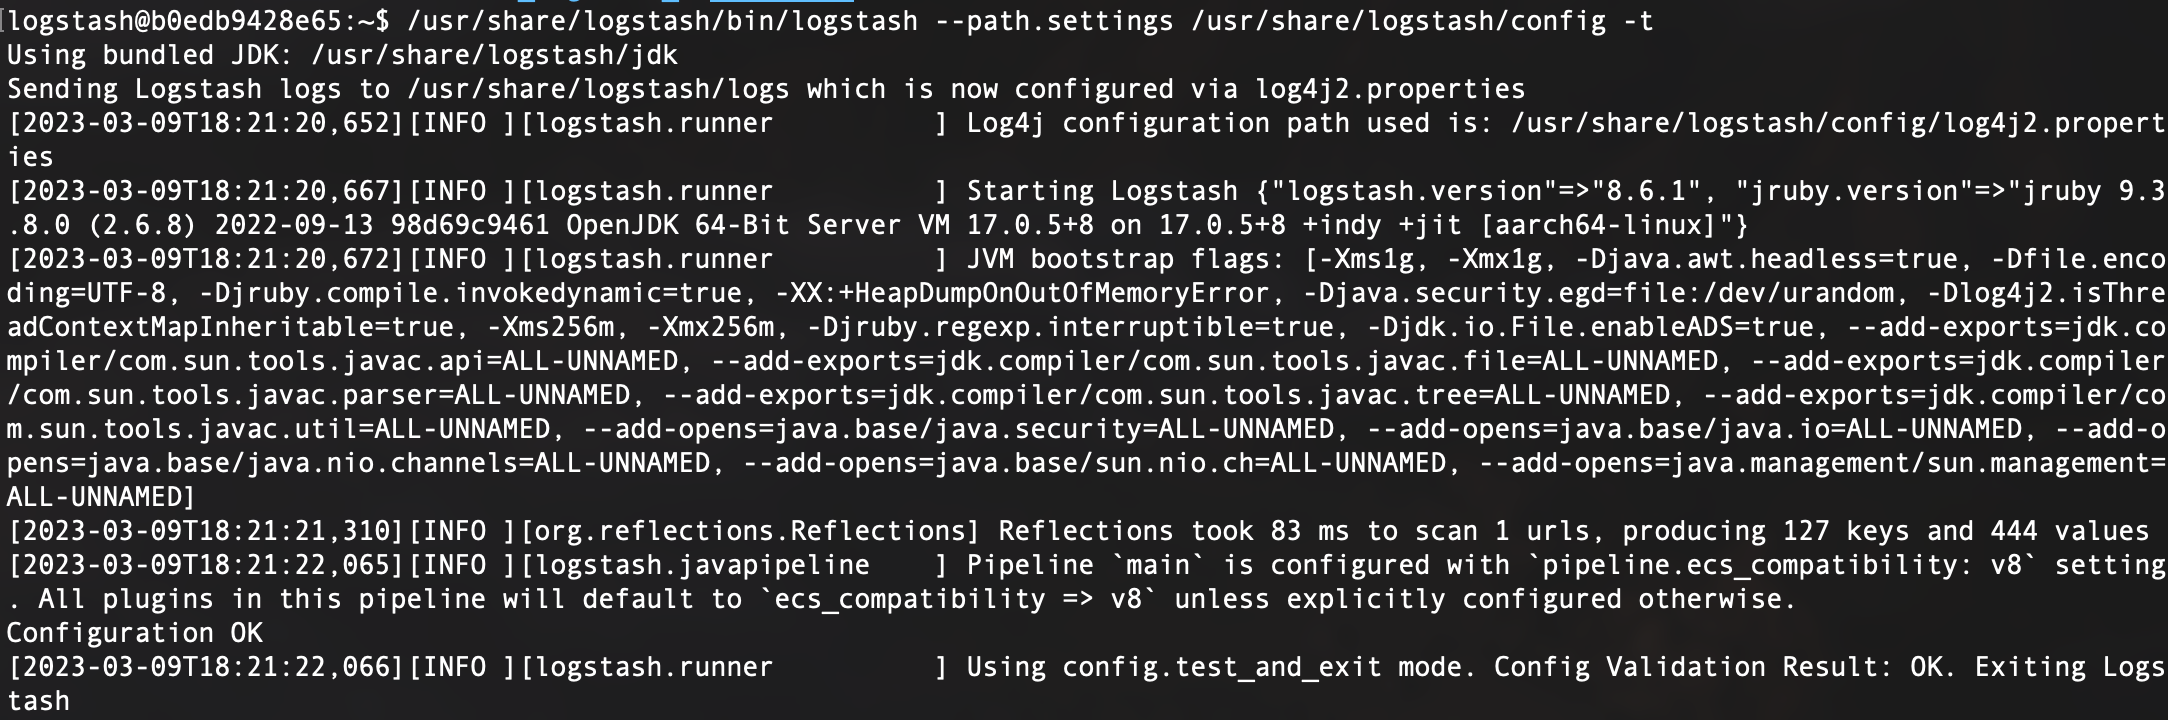
\includegraphics[width=\textwidth]{images/sc04.png} 

	\newpage

	\section*{Step 2}
	\noindent \textbf{Clone postgres repo}
	\begin{lstlisting}[style=fish]
git clone https://github.com/Digital-Media/postgres
cd postgres
	\end{lstlisting}

	\noindent \textbf{Create sql scripts in local folder named "scripts"} \\
	See \hyperref[listings:schema]{schema.sql} and \hyperref[listings:data]{data.sql} in appendix. \\

	\noindent \textbf{Map the scipts folder to the container adding scripts to the volumes:}
	\begin{lstlisting}[style=fish]
volumes:
  - ./scripts:/scripts
  - pgdata:/var/lib/postgresql/data
	\end{lstlisting}

	\noindent \textbf{Start postgres container with docker compose:}
	\begin{lstlisting}[style=fish]
docker compose -f docker-compose.yml up -d --build
	\end{lstlisting}

	\noindent \textbf{Open psql inside postgres container create schema and insert data:}
	\begin{lstlisting}[style=fish]
docker exec -it postgres psql -d postgres -U postgres
\i scripts/schema.sql
\i scripts/data.sql
	\end{lstlisting}

	\noindent \textbf{Download jdbc driver to local machine}
	\begin{lstlisting}[style=fish]
cd elk-stack-dock/logstash
mkdir jars
cd jars
curl -o postgresql-42.5.4.jar https://jdbc.postgresql.org/download/postgresql-42.5.4.jar
	\end{lstlisting}

	\noindent \textbf{Add this line to the end of the logstash Dockerfile}
	\begin{lstlisting}[style=fish]
COPY jars/* /usr/share/logstash/logstash-core/lib/jars/
	\end{lstlisting}

	\noindent \textbf{Run docker compose with build flag}
	\begin{lstlisting}[style=fish]
docker compose -f elk-stack-dock/docker-compose.yml up -d --build
	\end{lstlisting}

	\newpage

	\noindent \textbf{Test Postgres pipeline}
	\begin{lstlisting}[style=fish]
logstash --path.data data2 -e 'input {
  jdbc {
    jdbc_connection_string => "jdbc:postgresql://192.168.0.23:5432/postgres"
    jdbc_user => "postgres"
    jdbc_password => "geheim"
    jdbc_driver_class => "org.postgresql.Driver"
    statement => "SELECT * FROM order_item"
  }
} output {
  stdout {}
}'
	\end{lstlisting}
	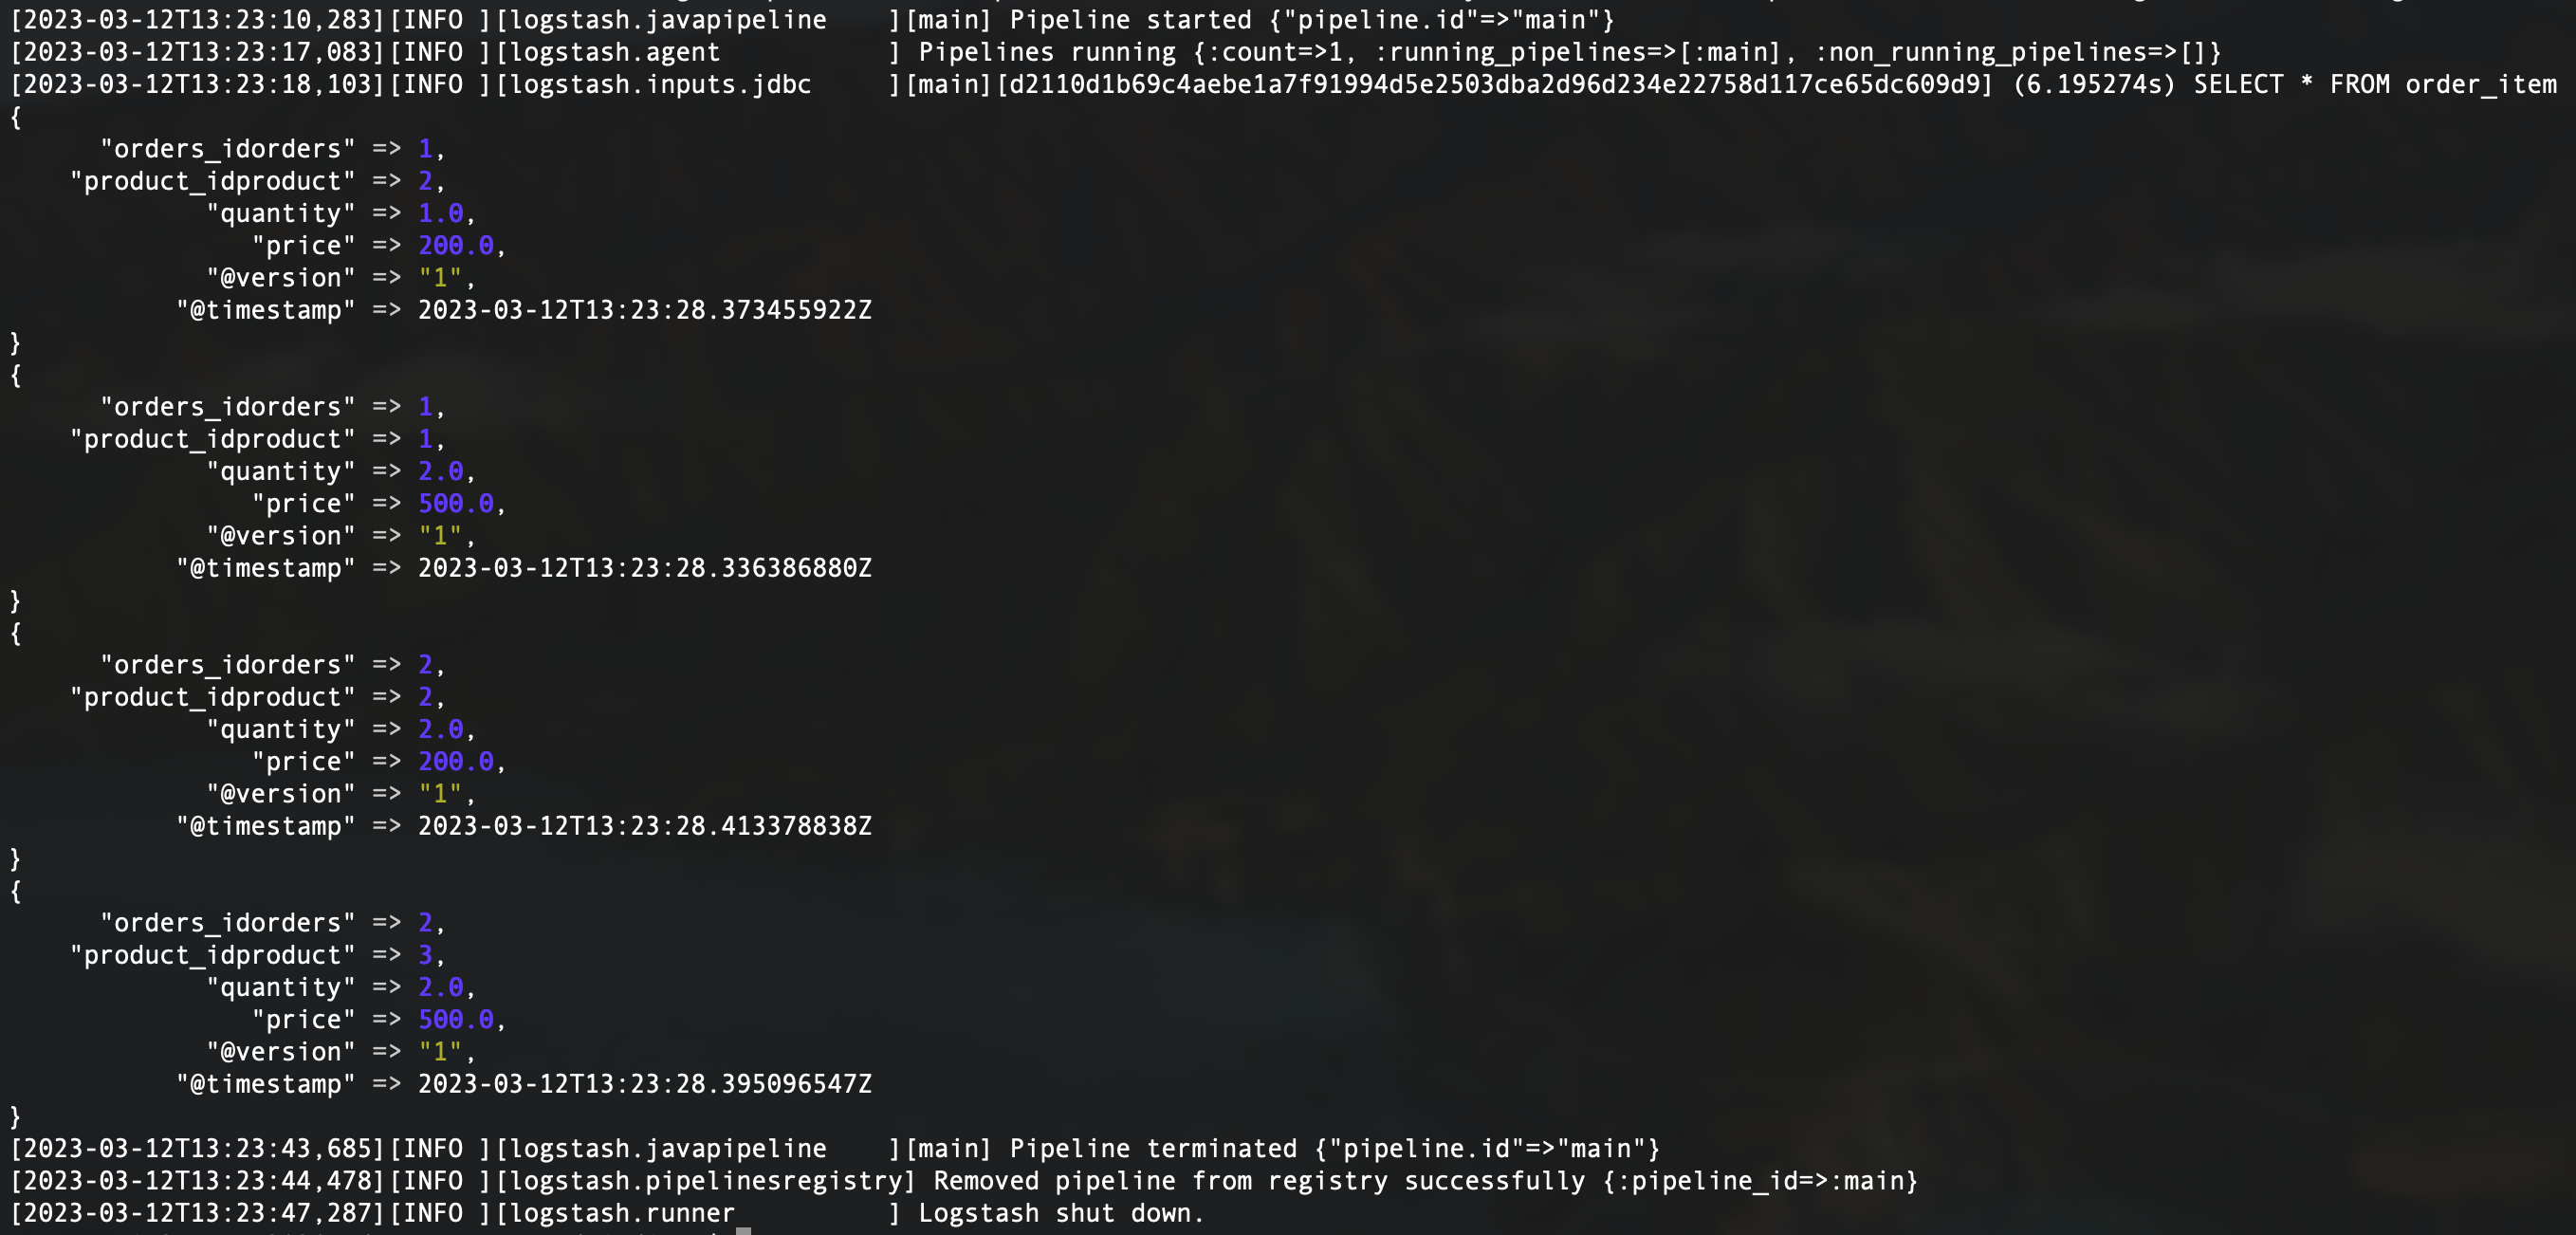
\includegraphics[width=\textwidth]{images/sc05.png} 

	\noindent \textbf{Write the new pipeline in the pipeline configuration file:} \\
	See \hyperref[listings:pipeline]{pipeline.conf} in appendix for the pipeline 
	\begin{lstlisting}[style=fish]
nvim elk-stack-dock/logstash/pipeline/logstash.conf
	\end{lstlisting}

	\noindent \textbf{Restart the logstash container to apply the new configuration}
	\begin{lstlisting}[style=fish]
docker stop elk-stack-dock_logstash_1 && docker start elk-stack-dock_logstash_1
	\end{lstlisting}

	\newpage
	\noindent \textbf{Check the logstash docker logs:}
	\begin{lstlisting}[style=fish]
docker logs -f elk-stack-dock_logstash_1
	\end{lstlisting}
	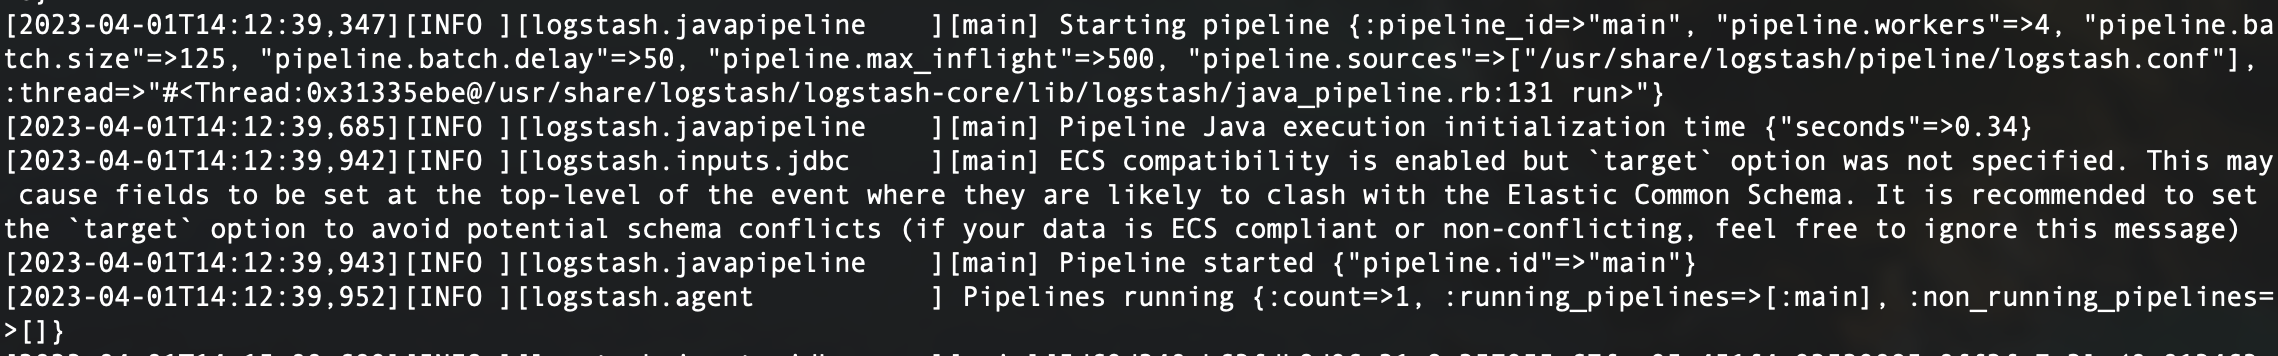
\includegraphics[width=0.9\textwidth]{images/sc06.png} 

	\noindent \textbf{Check the data in kibana} \\
	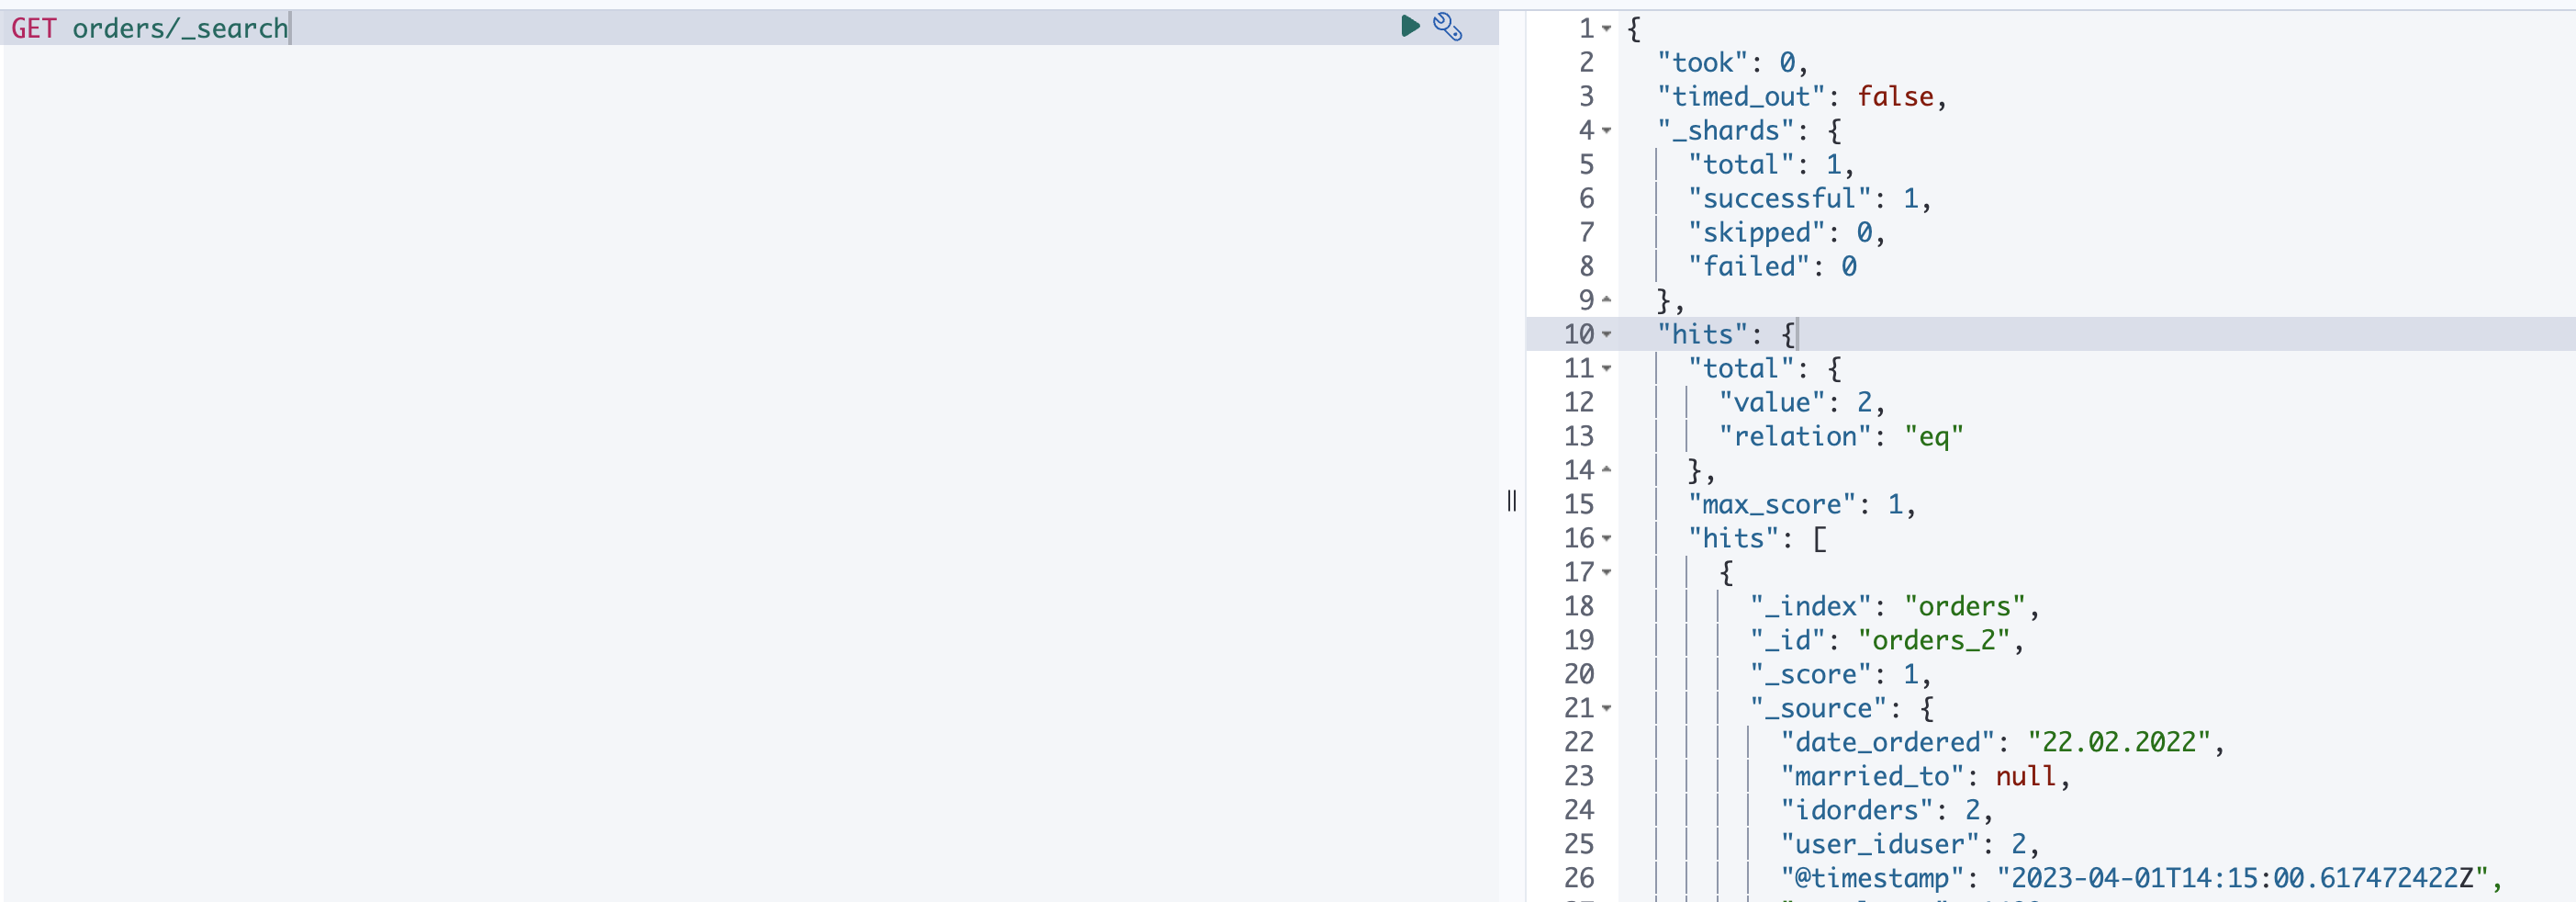
\includegraphics[width=0.9\textwidth]{images/sc07.png}  \\
	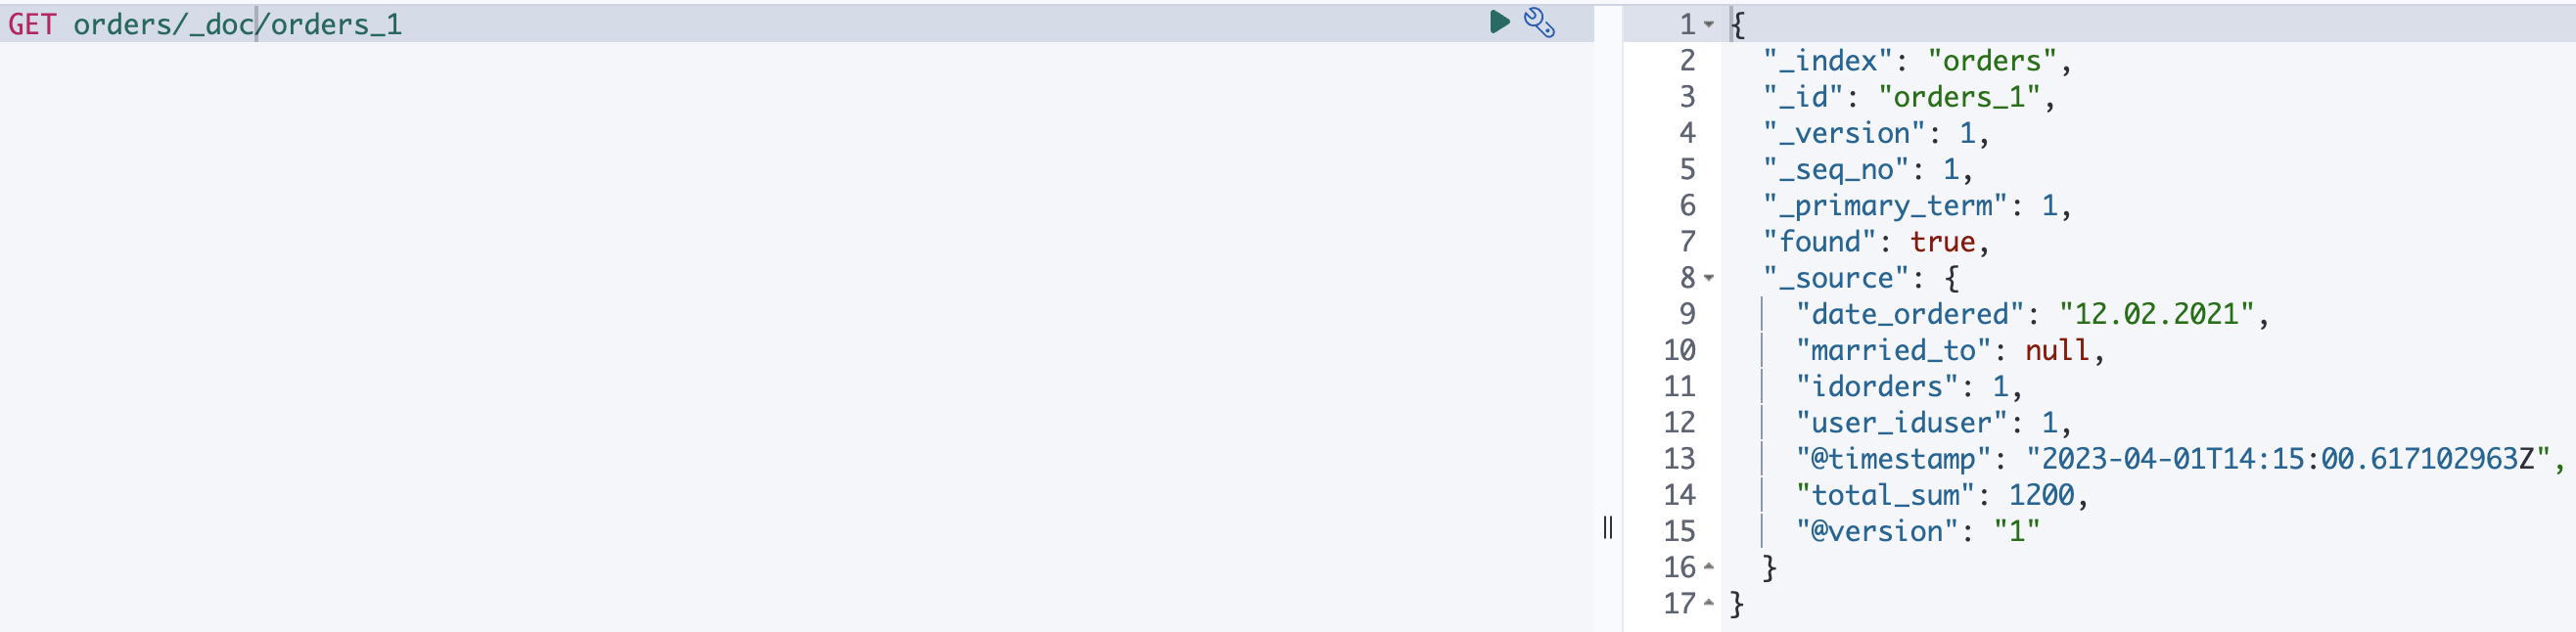
\includegraphics[width=0.9\textwidth]{images/sc08.png} 

	\noindent \textbf{Add a new sql entry (between 14:45 and 14:50) then check logs -> the data in es is updated every 5 minutes:}
	\begin{lstlisting}[style=fish]
docker exec -it postgres psql -d postgres -U postgres
INSERT INTO orders (idorders, user_iduser, total_sum, date_ordered) VALUES (3, 2, 1400, '23.02.2022');
	\end{lstlisting}
	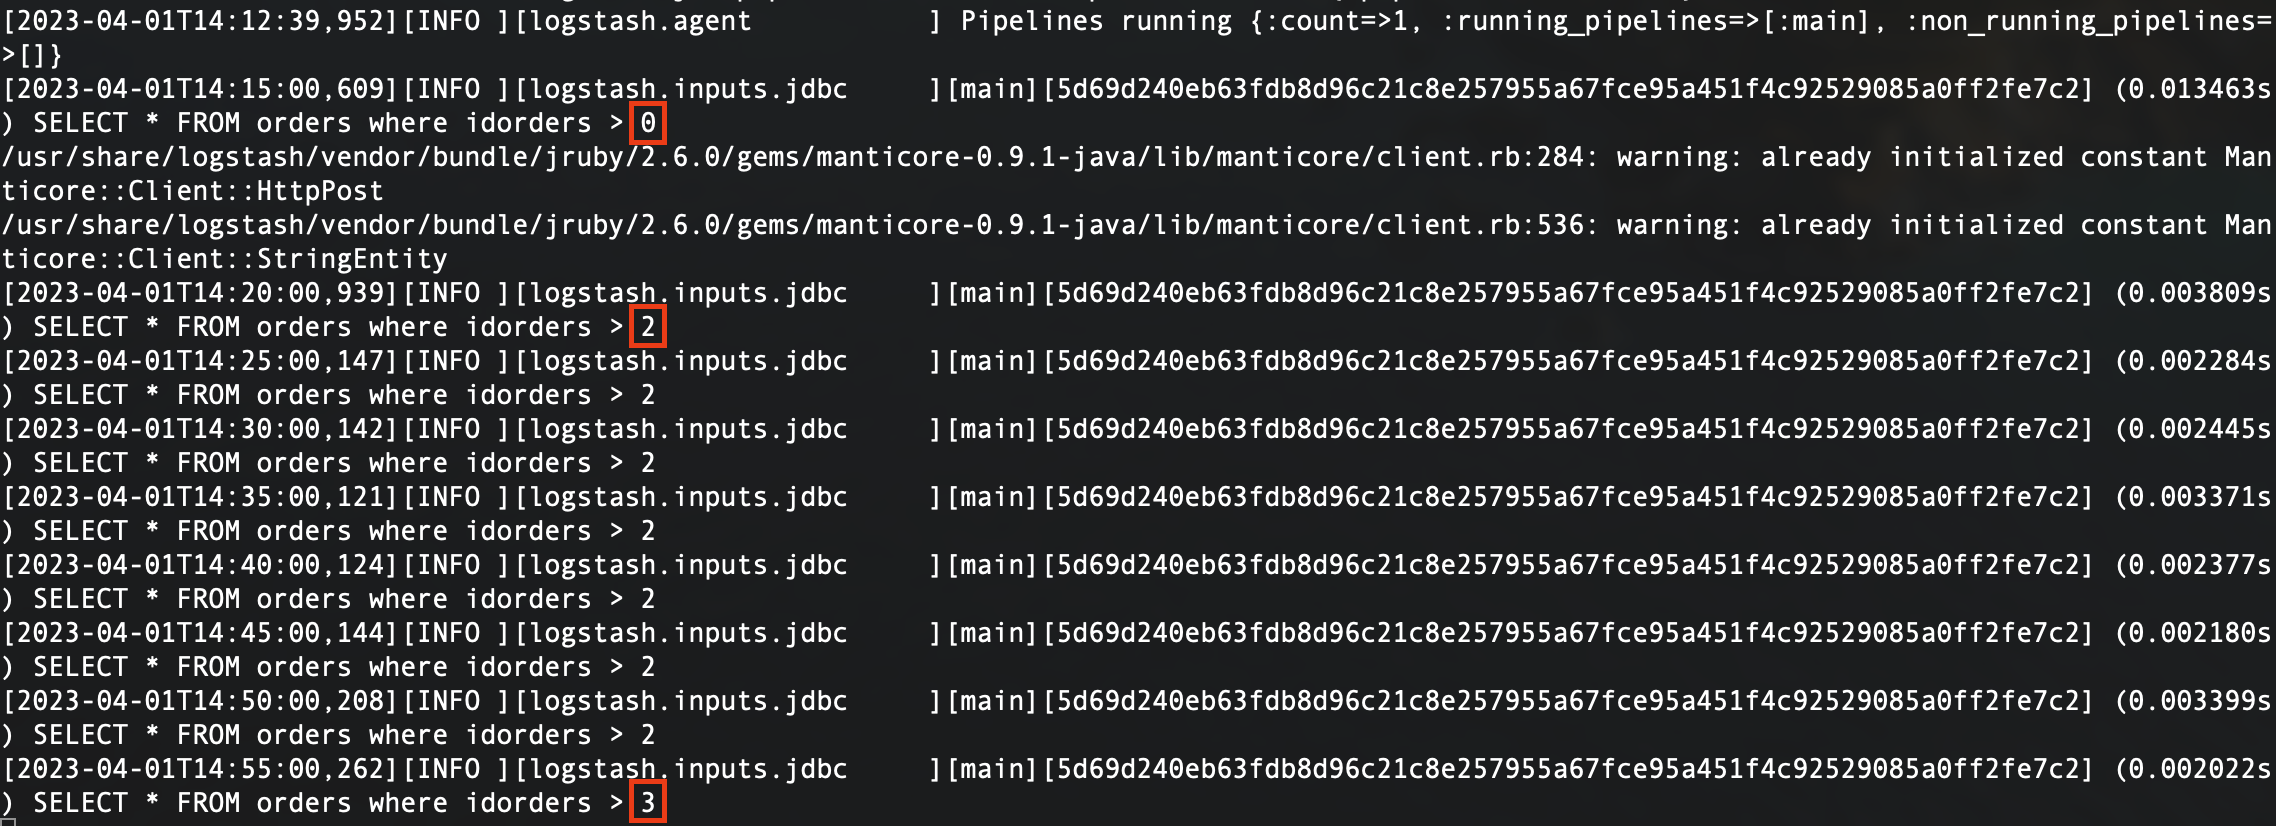
\includegraphics[width=0.9\textwidth]{images/sc09.png} 
	\newpage

	\noindent \textbf{Logstash pipeline vs. MongoDB pipeline} \\
	MongoDB supports a way to import data from files e.g. json files using mongoimport.
	The same workflow that we implemented using logstash contains this steps using MongoDB and mongoimport:
	\begin{enumerate}[noitemsep]
		\item Check which data is already synced to the MongoDB e.g. storing the last synced id
		\item Export the "new" data from postgres to e.g. json file
		\item Import the json file using mongoimport
	\end{enumerate}

	\noindent 
	In my opinion this is not the perfect solution, because it means, that some code has to be written and maintained if this should be done automatically.
	Of course, it is not very complex to sequentially fetch the new data, convert it to json and write it into MongoDB.
	But writing the code for the pipeline and hosting the pipeline is much more error prone than just using and configuring a tool like logstash.

	Still I would not decide to use ElasticSearch just because of the advantage of logstash compared to mongoimport.
	\newpage

	\section*{Step 3}
	\noindent \textbf{Start Metricbeat}
	\begin{lstlisting}[style=fish]
docker-compose \
	docker-compose.yml \
	-f extensions/metricbeat/metricbeat-compose.yml \
	up -d
	\end{lstlisting}

	\noindent \textbf{Change the environments in the \hyperref[listings:envs]{.env} file} \\
	See the file \hyperref[listings:envs]{.env} file in the appendix.
	\begin{lstlisting}[style=fish]
nvim elk-stack-dock/.env
	\end{lstlisting}

	\noindent \textbf{Run the setup container again}
	\begin{lstlisting}[style=fish]
docker compose -f docker-compose.yml rm setup 
docker volume rm elk-stack-dock_setup 
docker-compose -f docker-compose.yml up setup
	\end{lstlisting}

	\noindent \textbf{Check Kibana logs => http server running at...} \\
	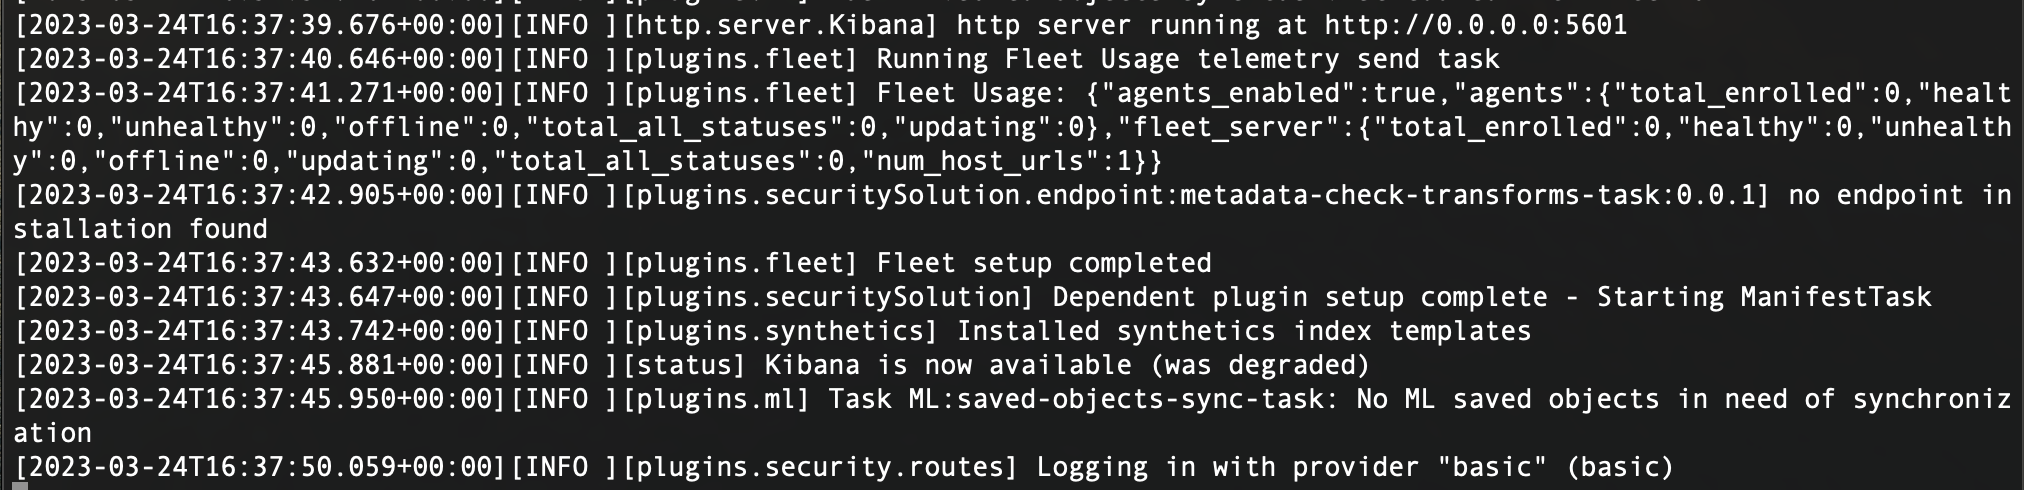
\includegraphics[width=\textwidth]{images/sc10.png}

	\noindent \textbf{Restart metricbeat (as soon as Kibana is ready)}
	\begin{lstlisting}[style=fish]
docker-compose \
	-f docker-compose.yml \
	-f extensions/metricbeat/metricbeat-compose.yml \
	restart metricbeat
	\end{lstlisting}

	\newpage

	\noindent \textbf{Check metricbeat data in Kibana} \\ \\
	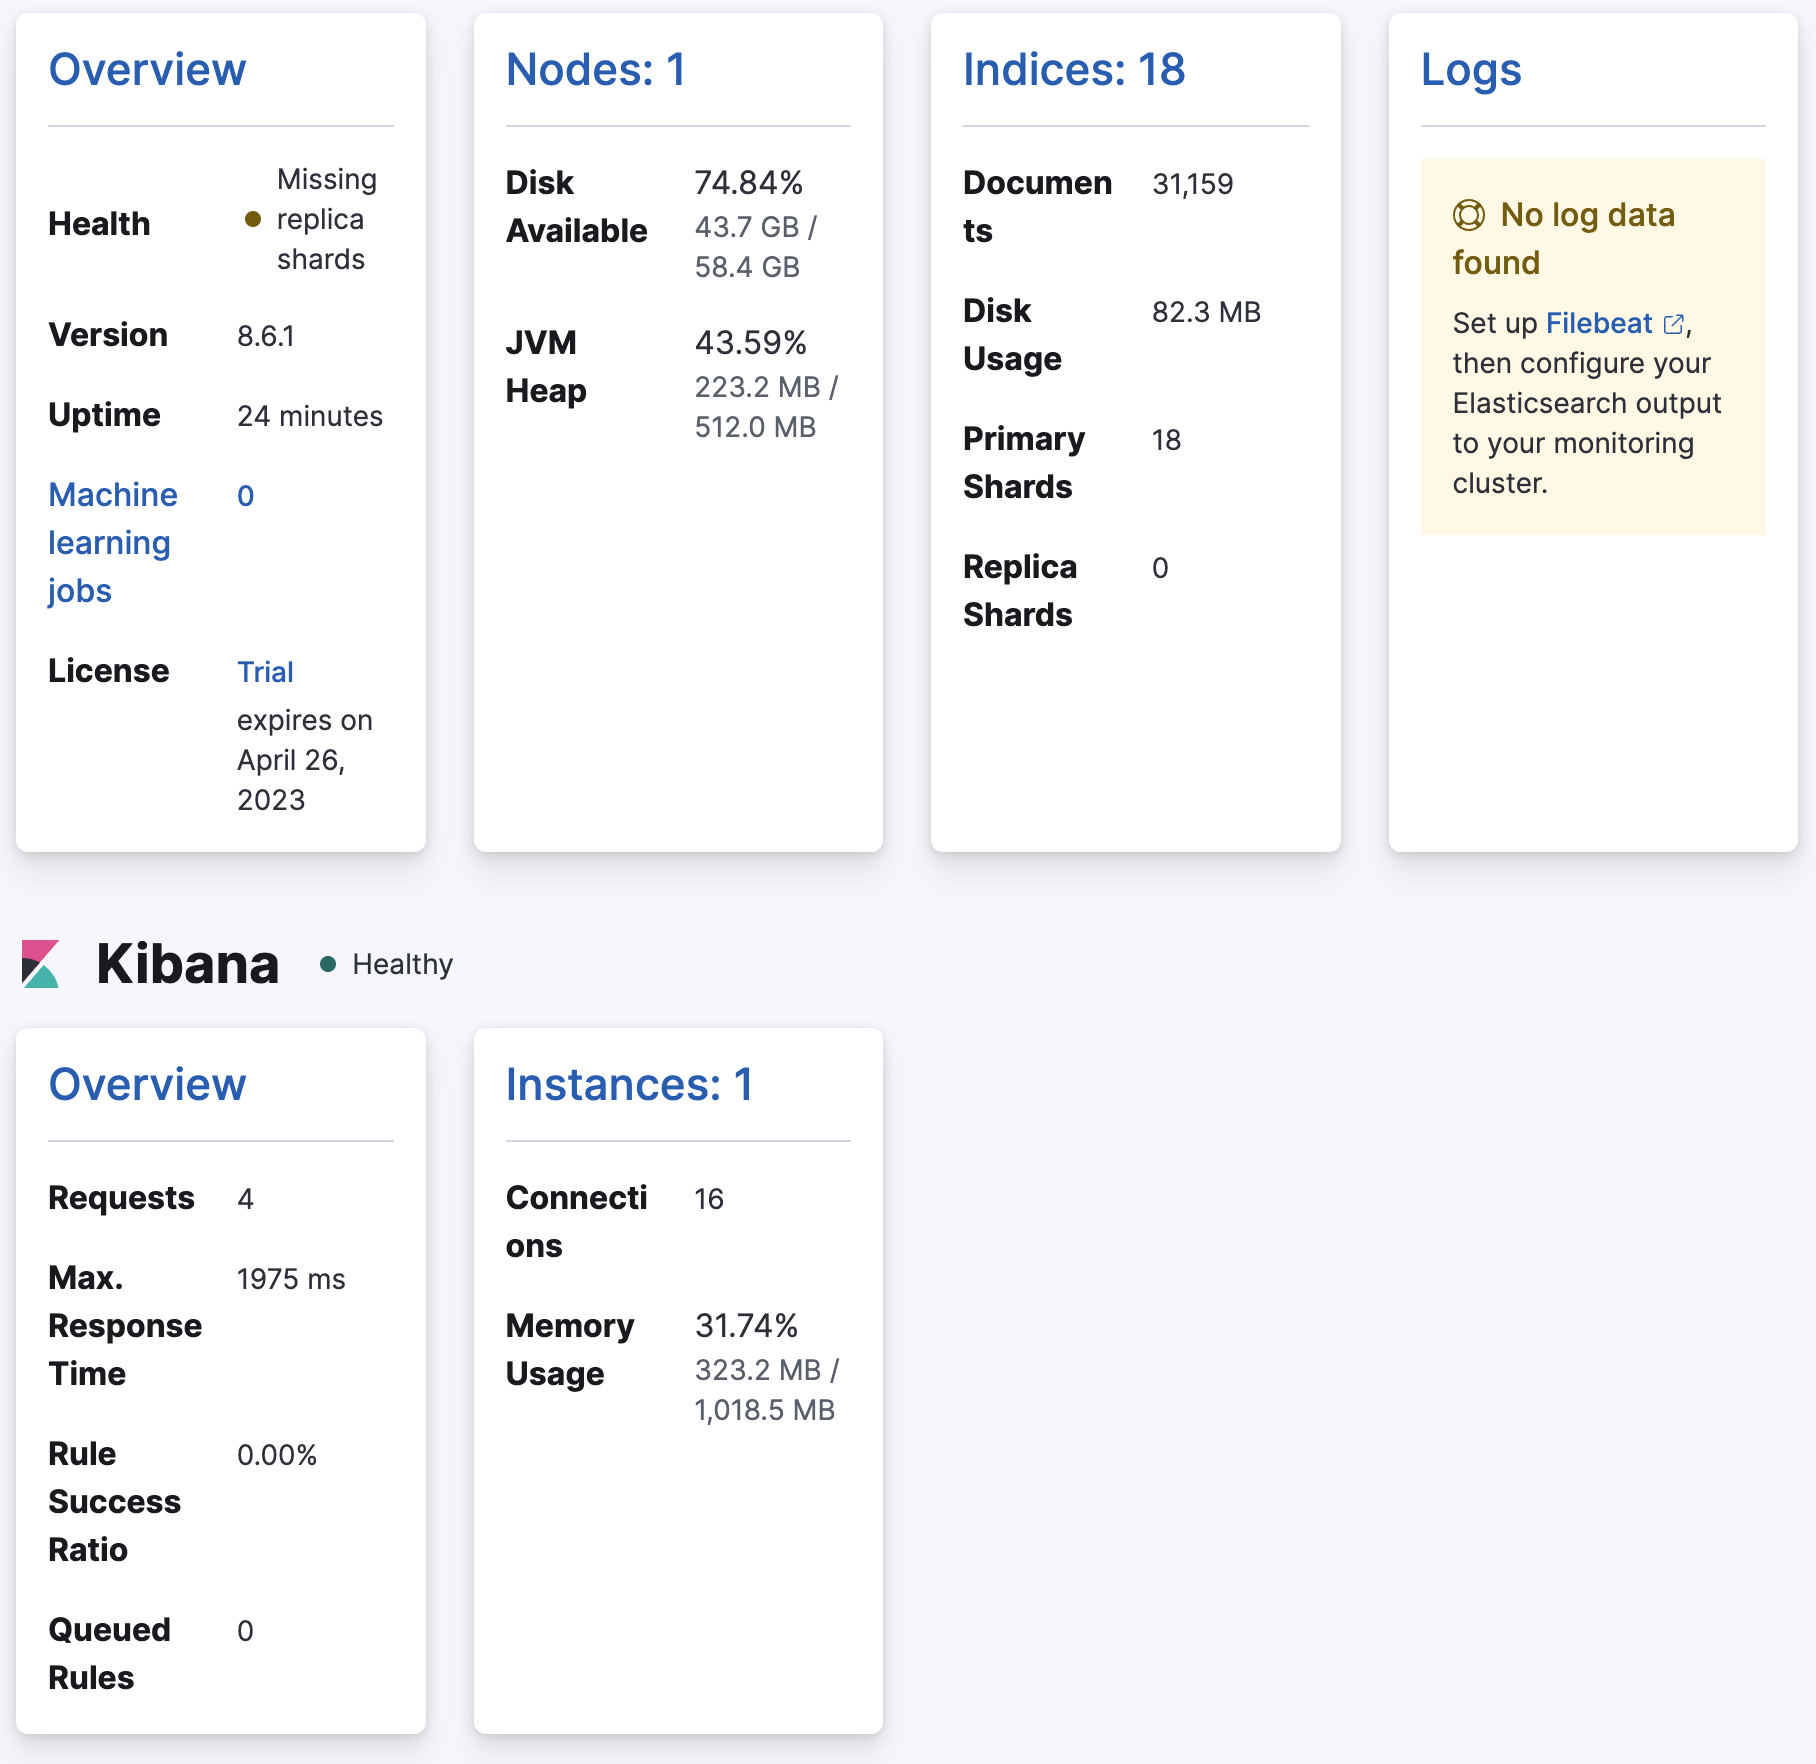
\includegraphics[height=0.45\textheight]{images/sc12.png} \\
	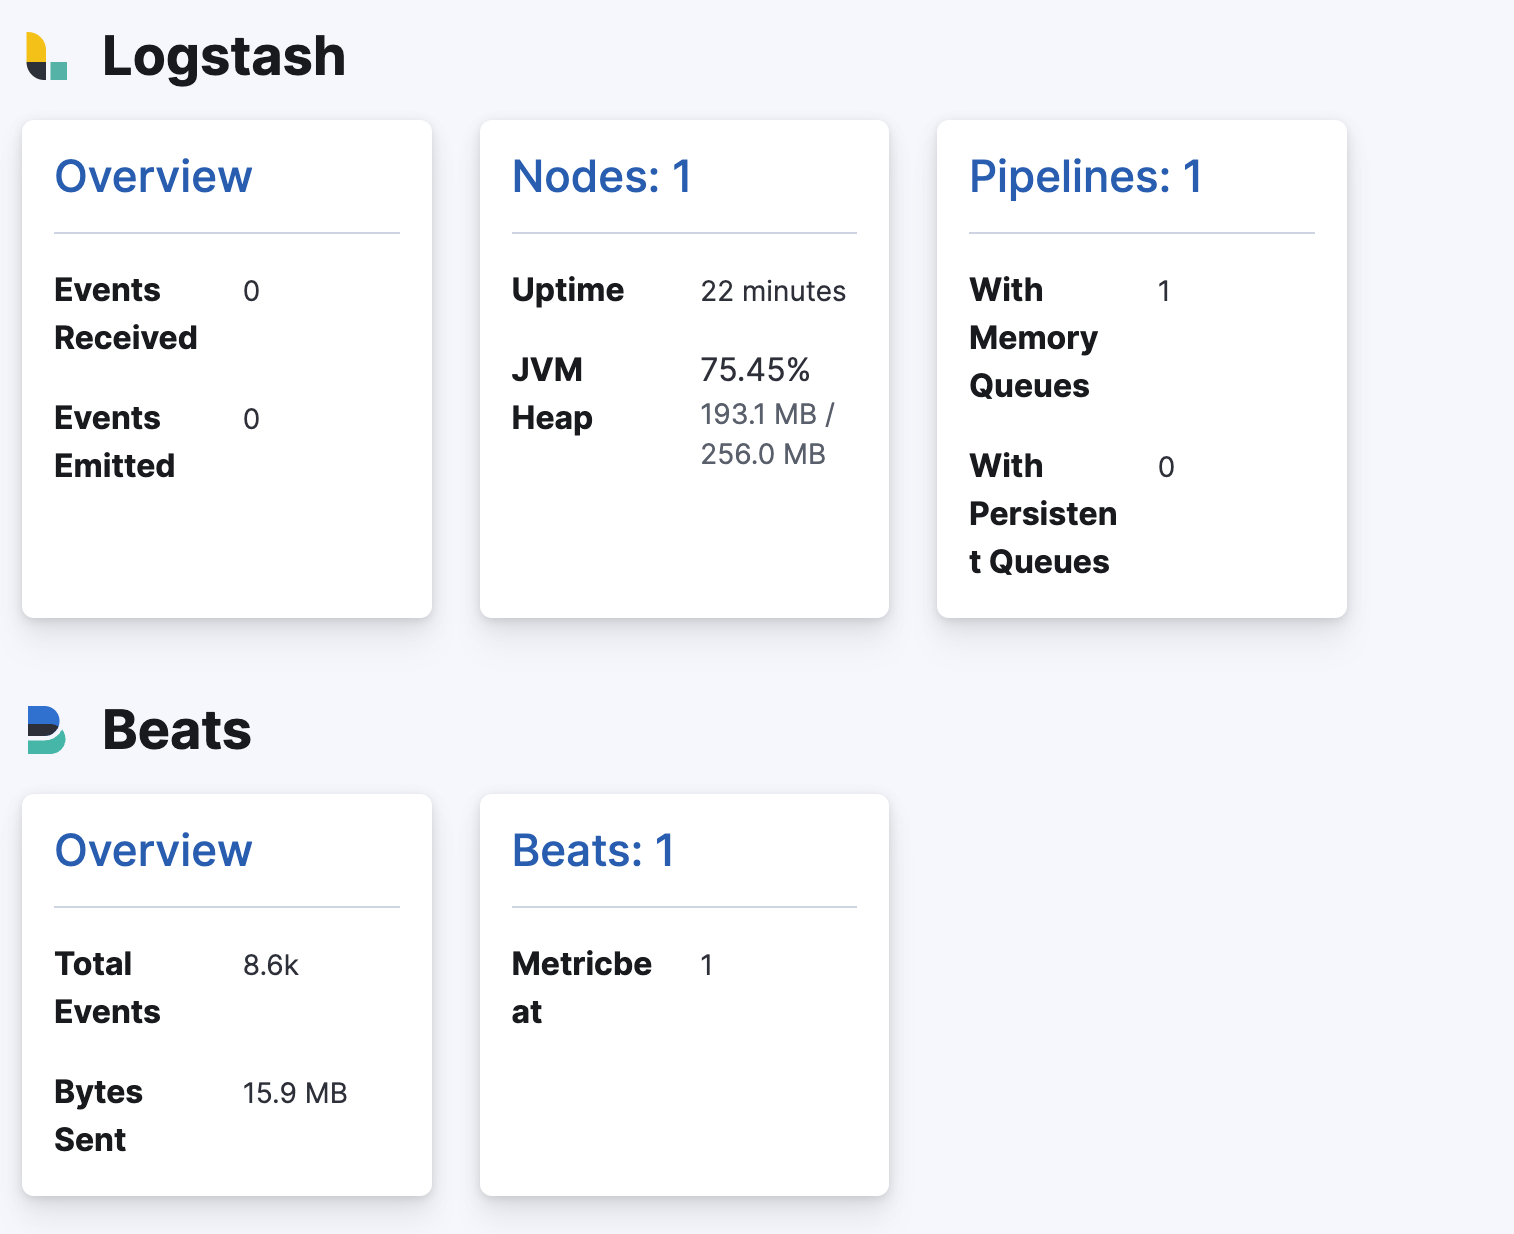
\includegraphics[height=0.45\textheight]{images/sc13.png}
	
	\newpage

	\noindent \textbf{Retrieve data using curl} \\
	Please write me if you need the files response1.json and response2.json.
	I did not hand them in because we can upload only one document in moodle, and I guess the screenshots show the most important parts.
	\begin{lstlisting}[style=fish]
curl -X GET -u elastic:changeme "http://localhost:9200/_search?pretty" > response1.json && head -n20 response1.json
	\end{lstlisting}
	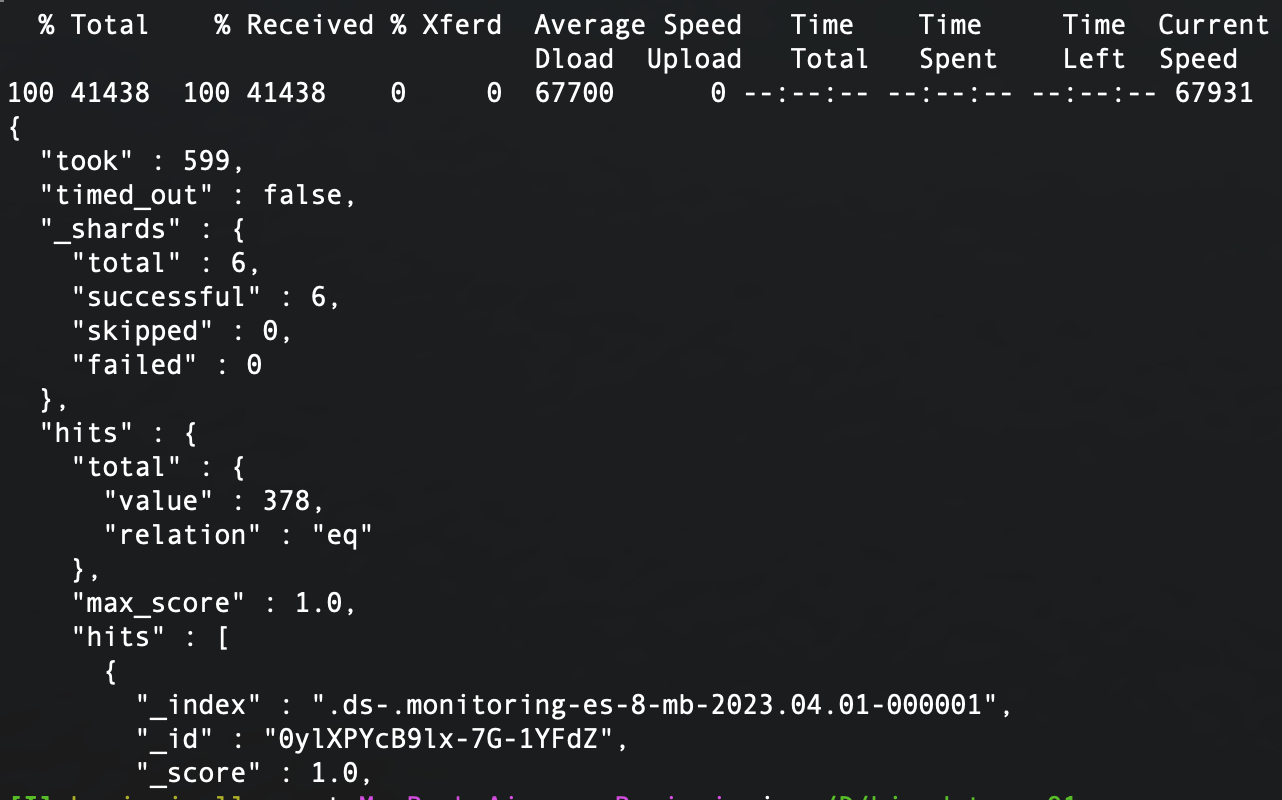
\includegraphics[height=0.32\textheight]{images/sc14.png}

	\begin{lstlisting}[style=fish]
curl -X GET -u elastic:changeme "http://localhost:9200/orders/_search?pretty" > response2.json && head -n20 response2.json
	\end{lstlisting}
	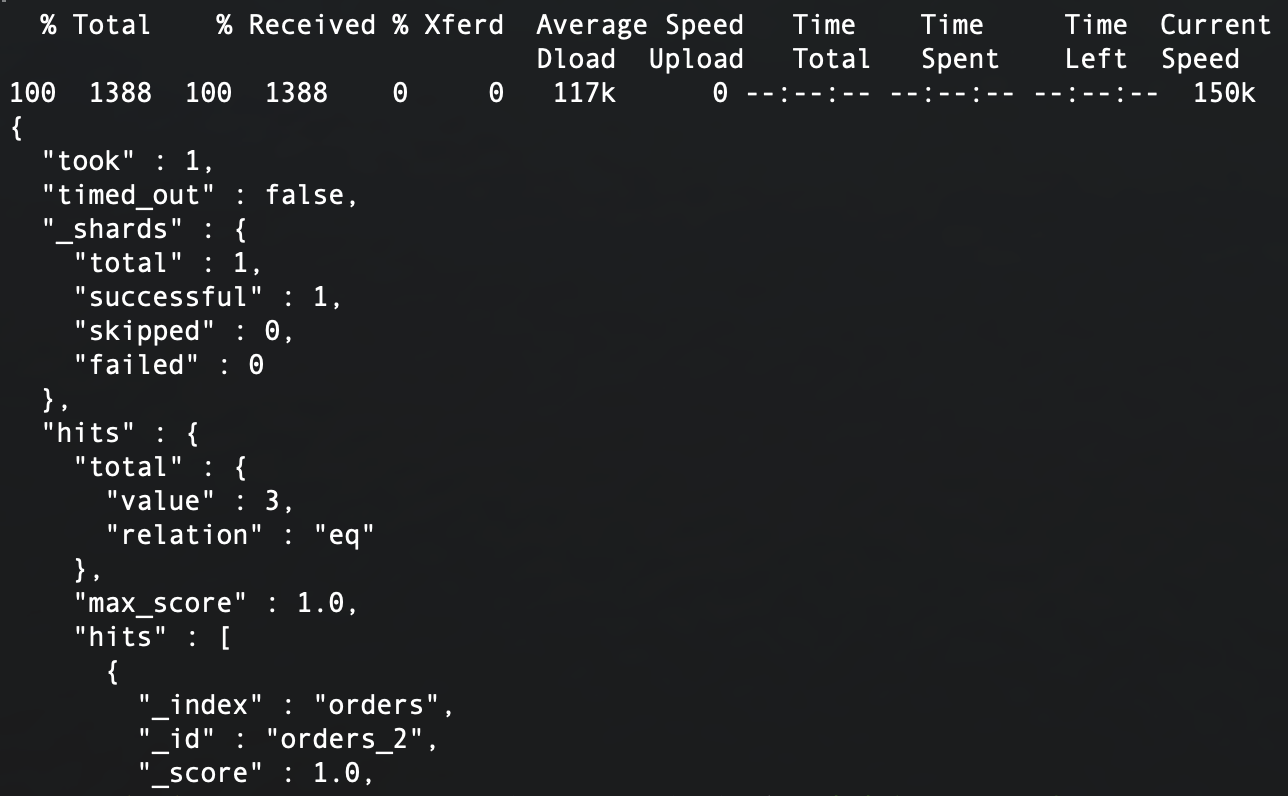
\includegraphics[height=0.32\textheight]{images/sc15.png}

	\newpage

	\noindent \textbf{Match specific entry} \\
	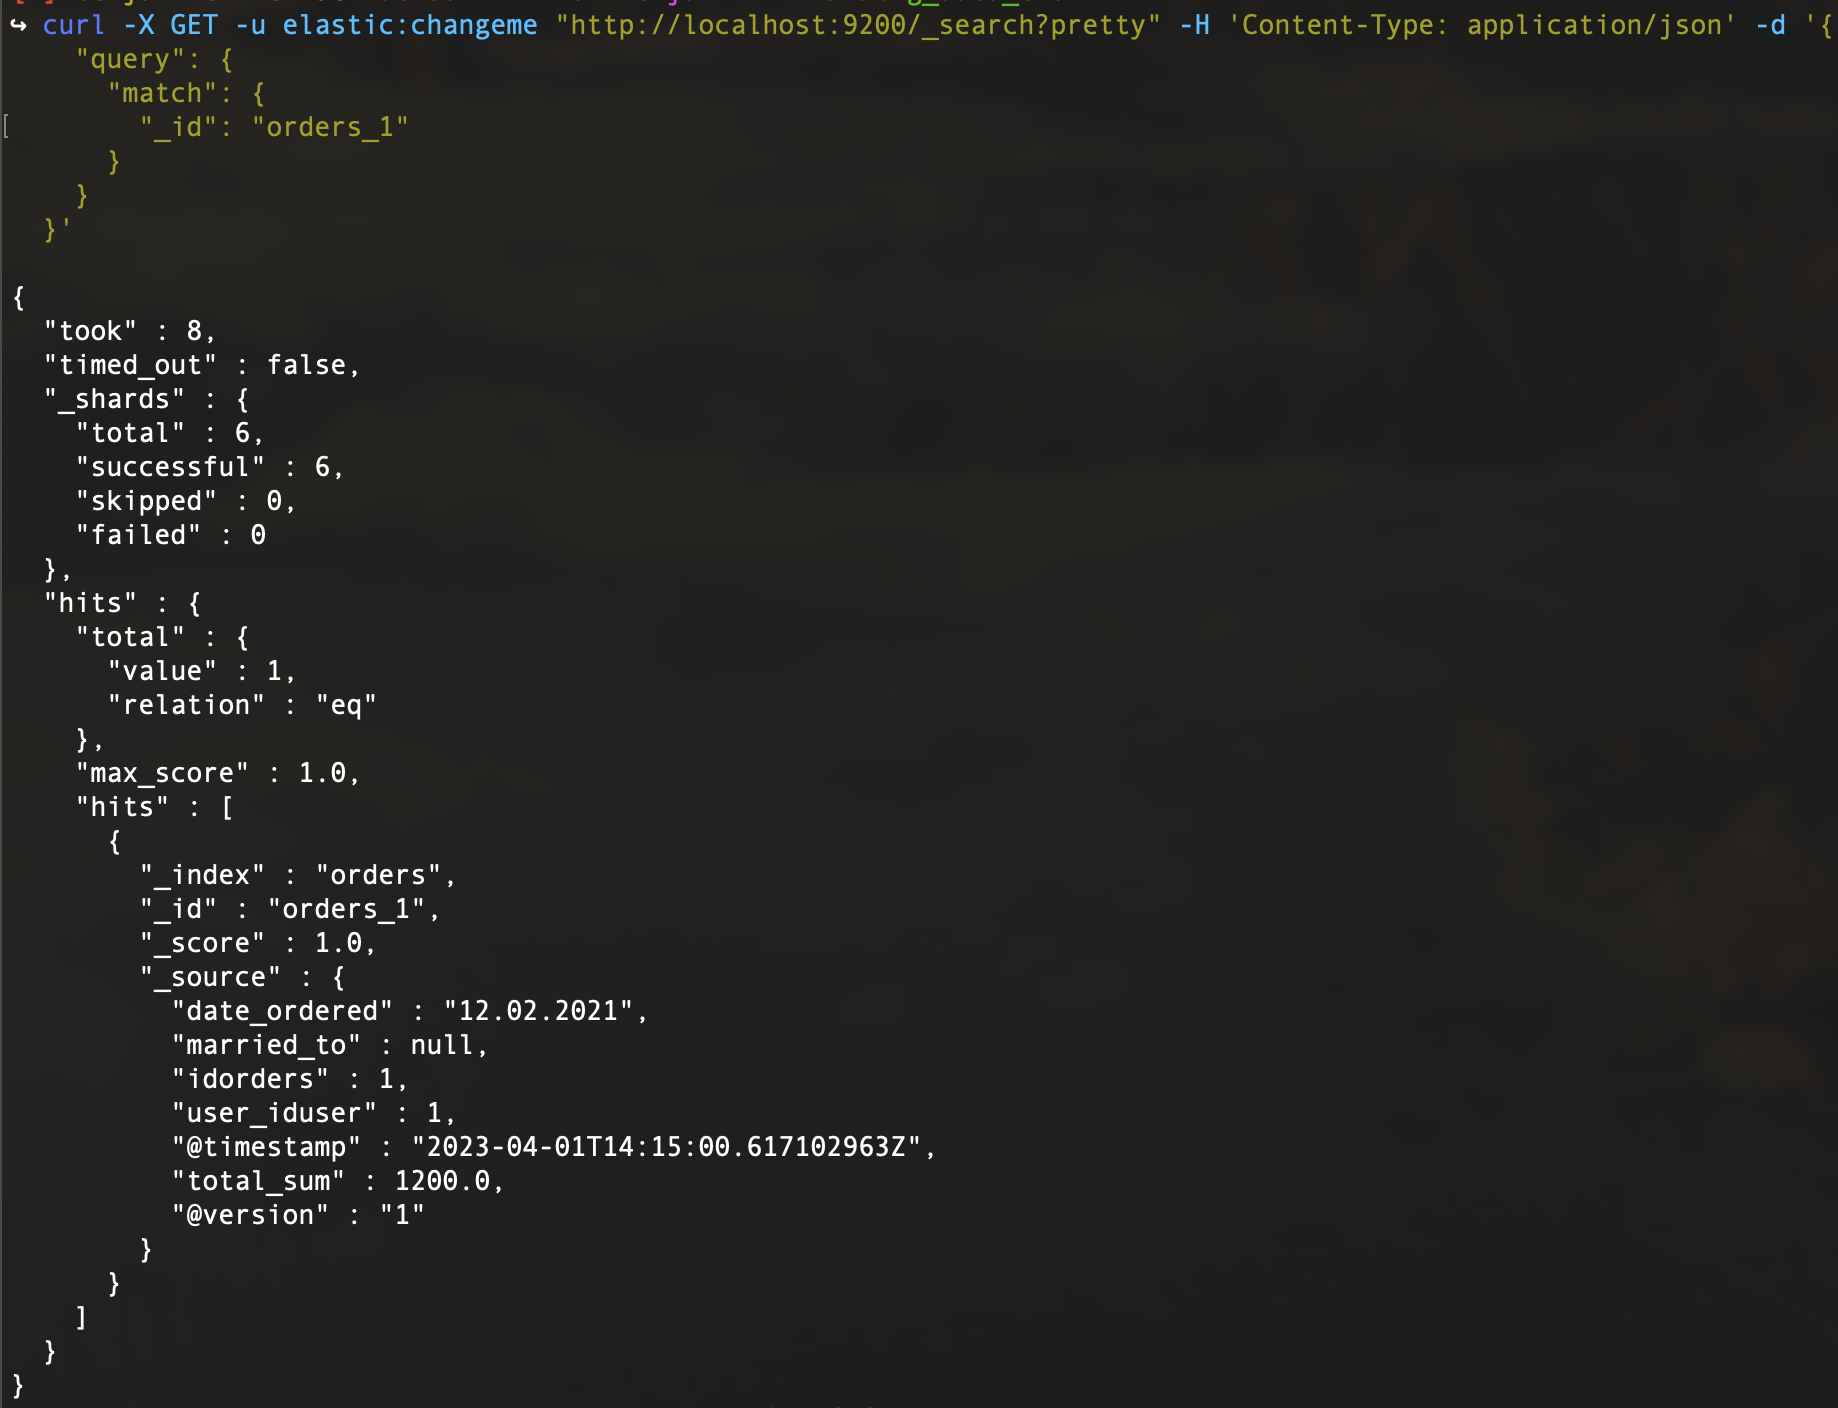
\includegraphics[width=\textwidth]{images/exists.png}

	\noindent \textbf{Match entry that does not exist} \\
	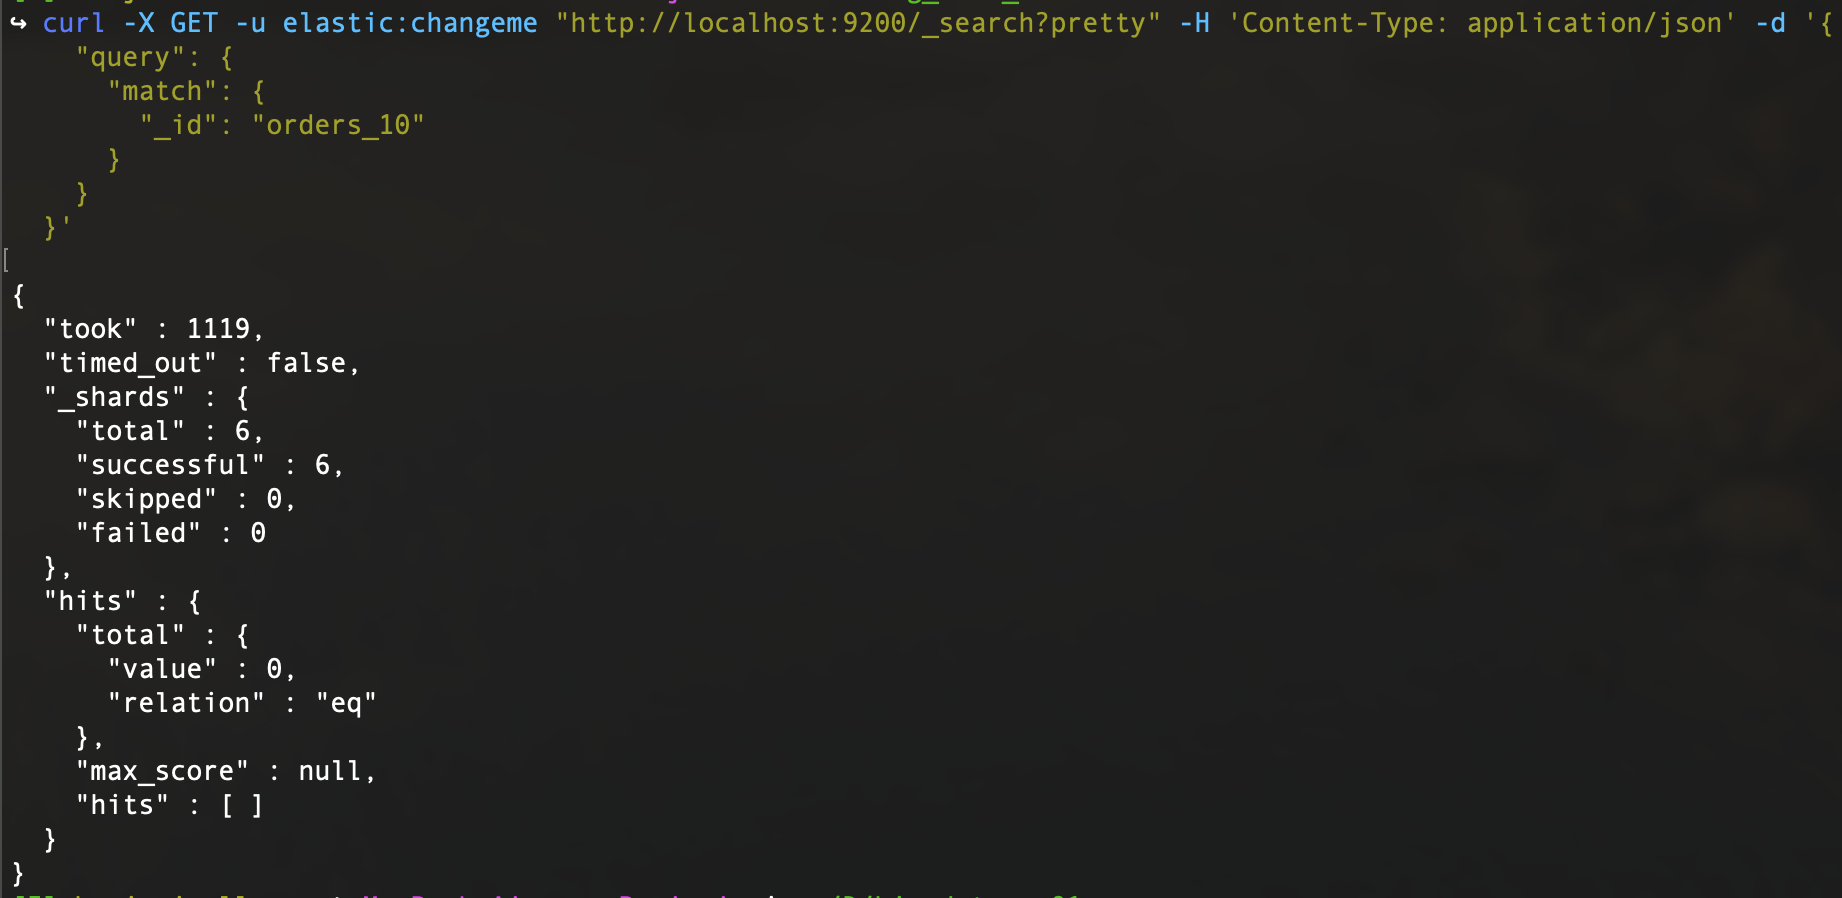
\includegraphics[width=\textwidth]{images/not_exists.png}

	\noindent \textbf{Query all entries in index without match condition} \\
	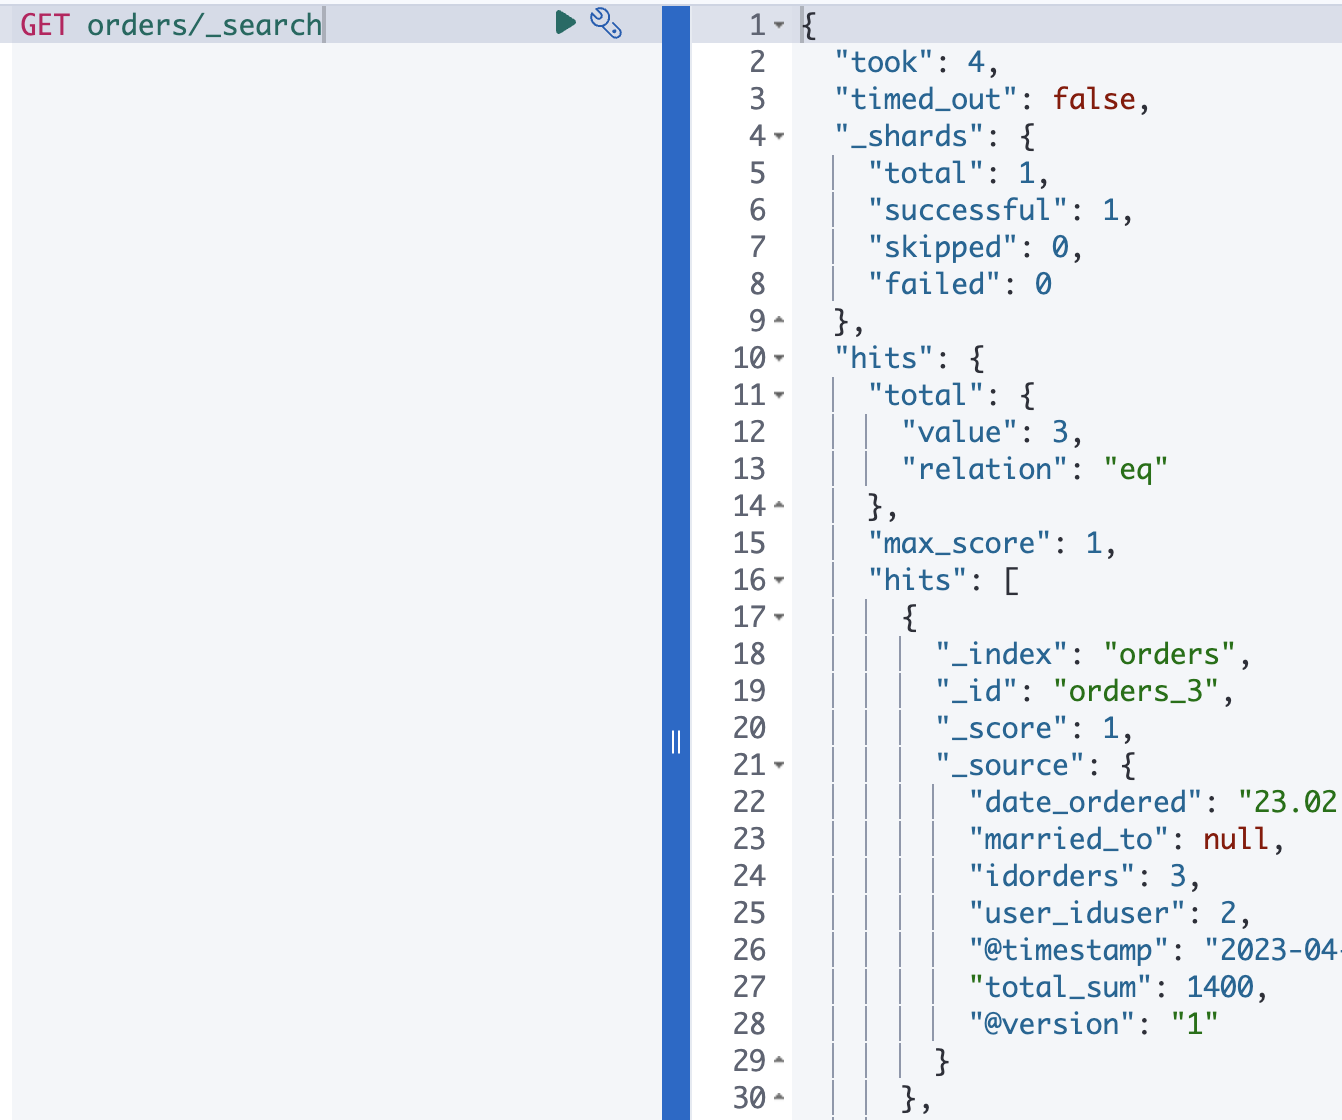
\includegraphics[height=0.42\textheight]{images/search_all.png}

	\noindent \textbf{Query all entries in index with match condition} \\
	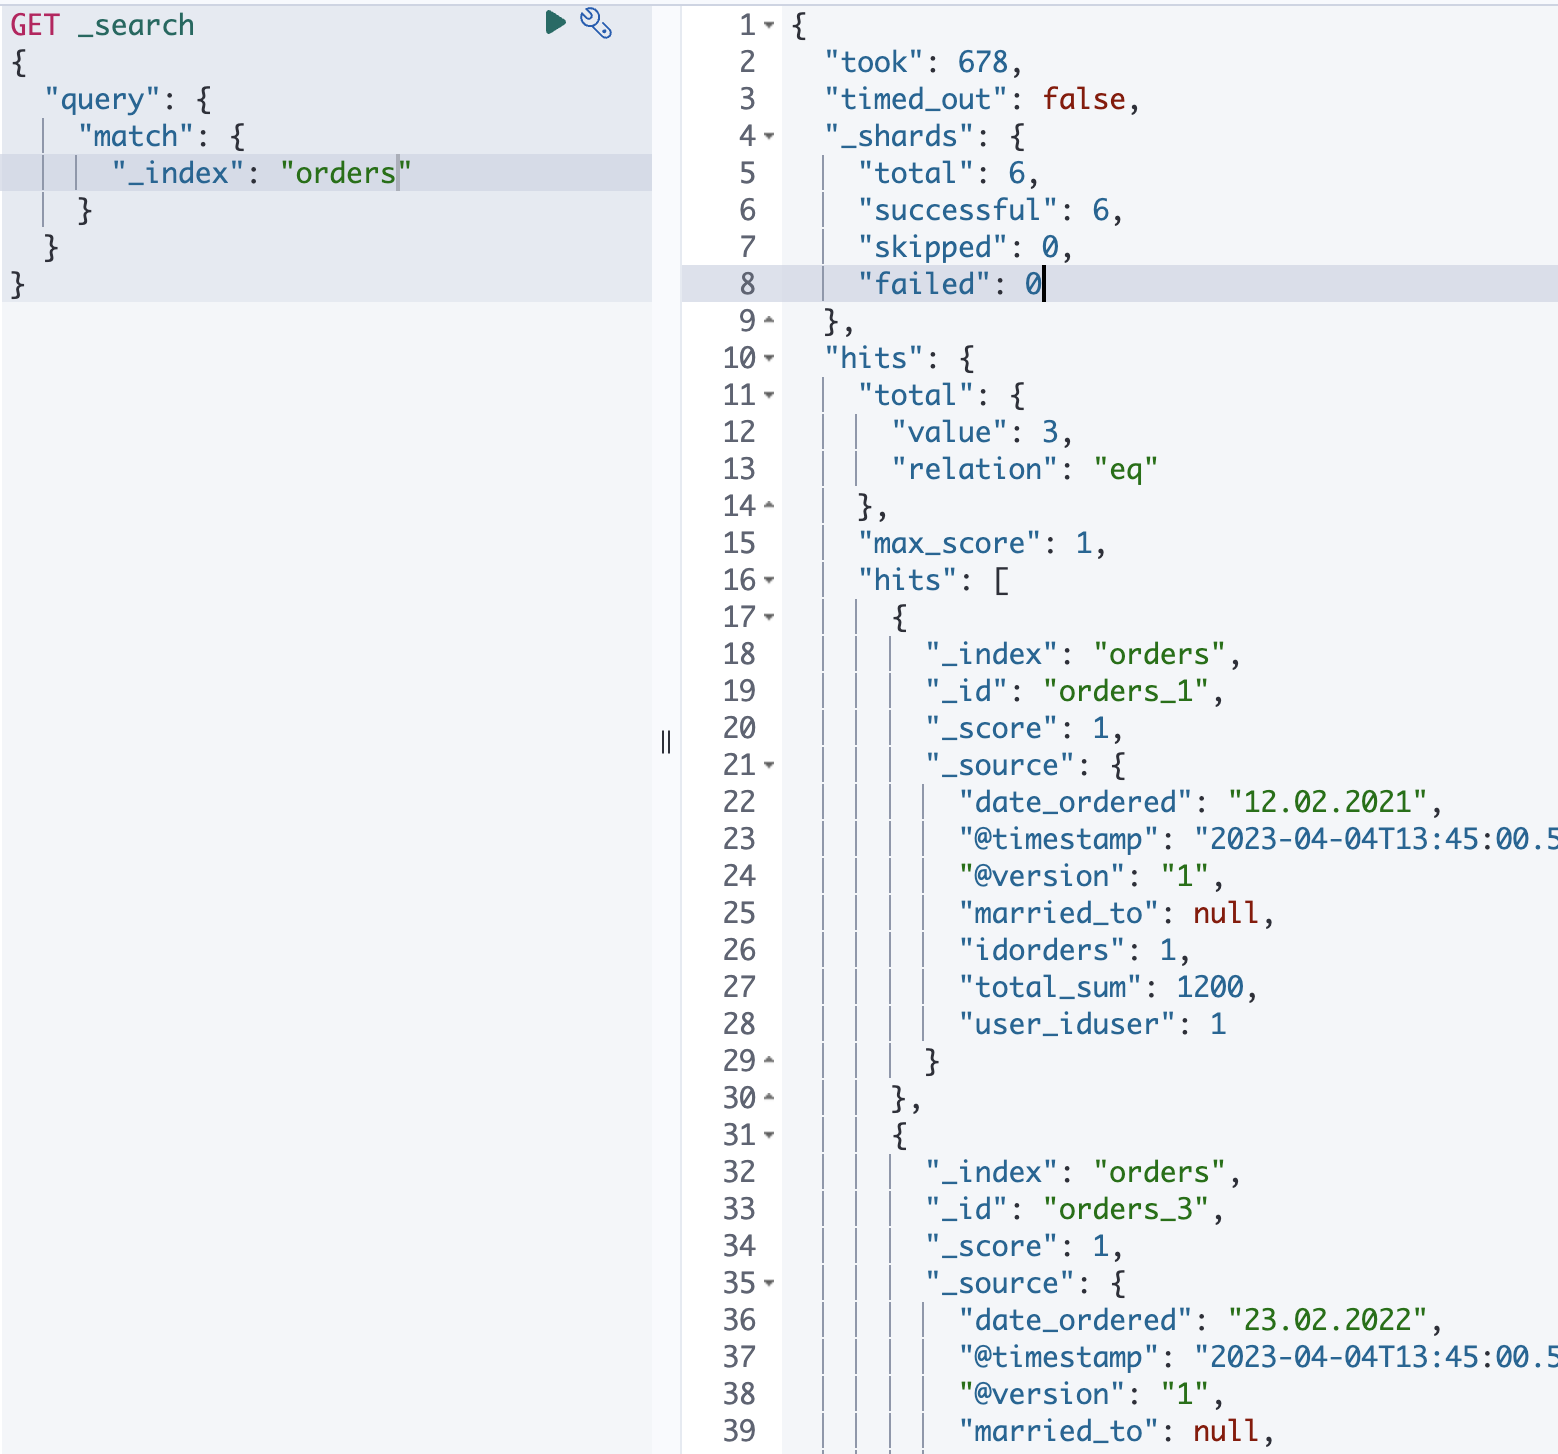
\includegraphics[height=0.47\textheight]{images/search_all_match.png}

	\newpage

	\noindent \textbf{Query specific entry without match condition} \\
	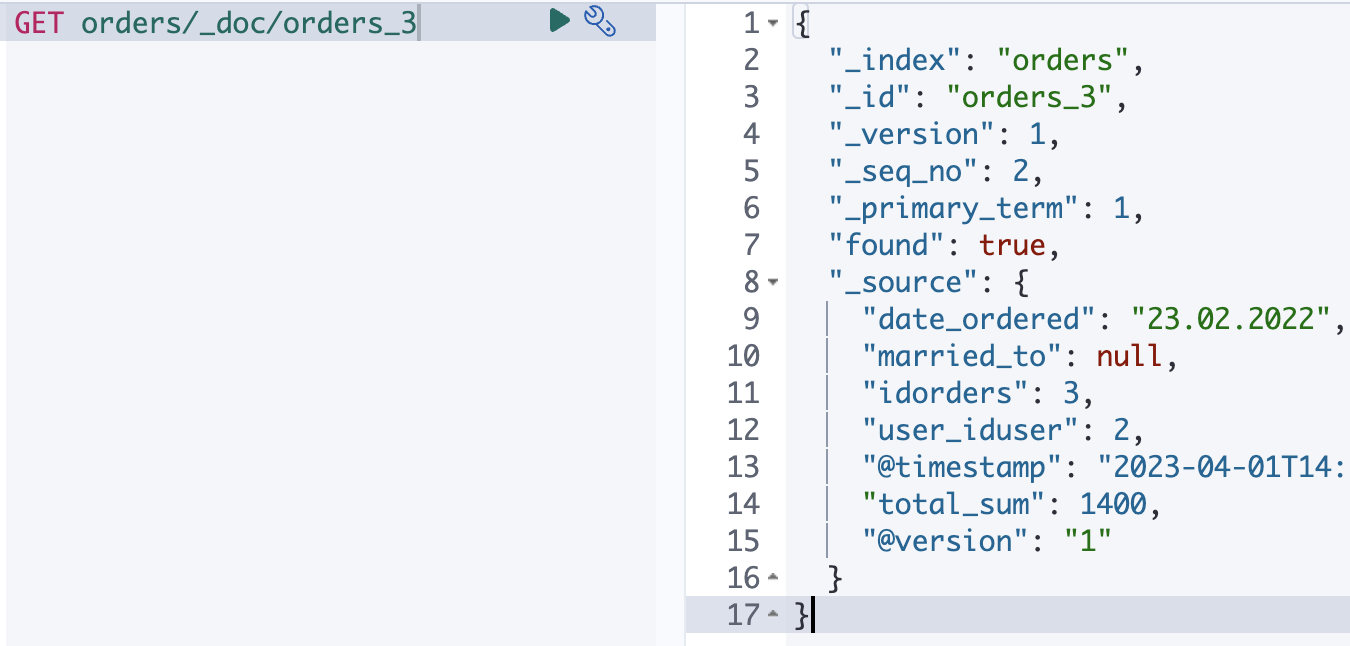
\includegraphics[width=\textwidth]{images/search_one.png}

	\noindent \textbf{Query specific entry with match condition} \\
	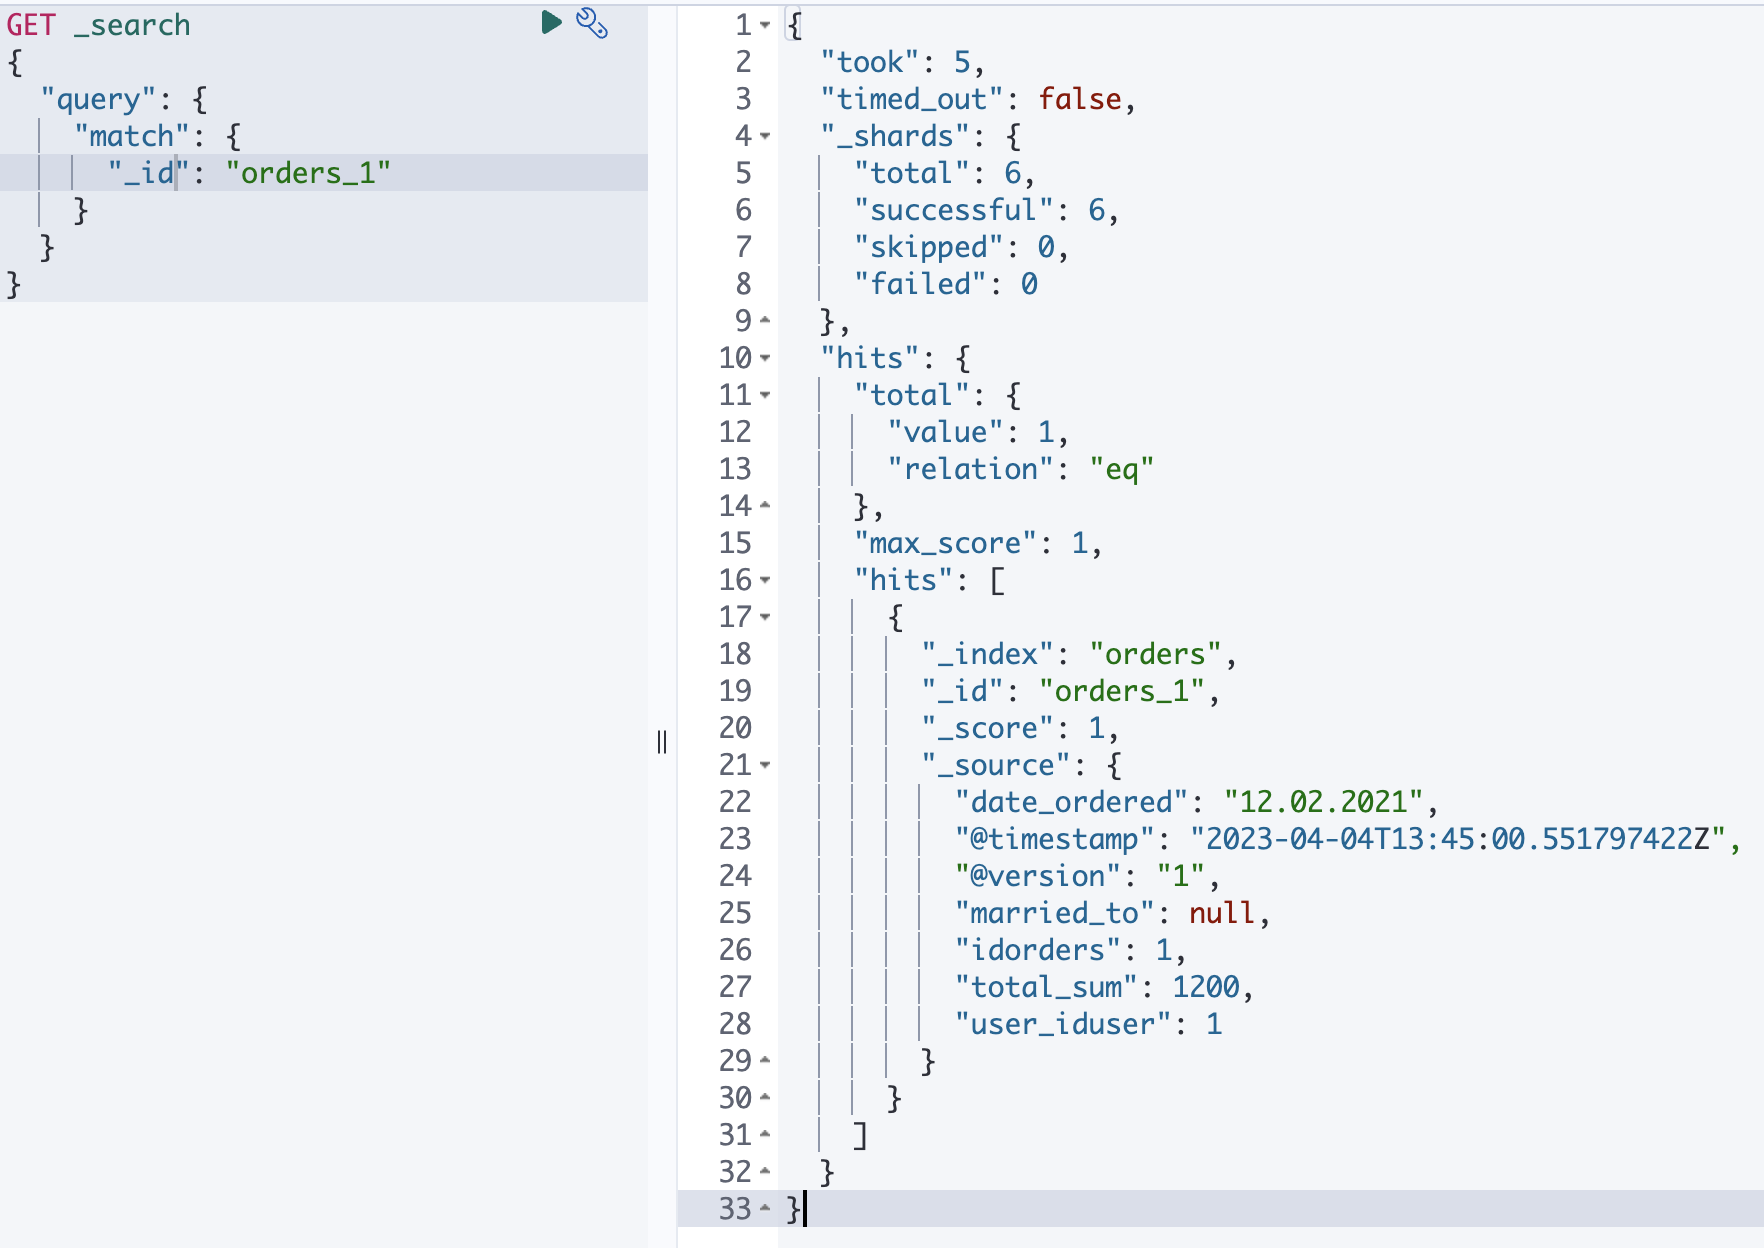
\includegraphics[width=\textwidth]{images/search_one_match.png}

	\newpage

	\noindent \textbf{Sort asc} \\
	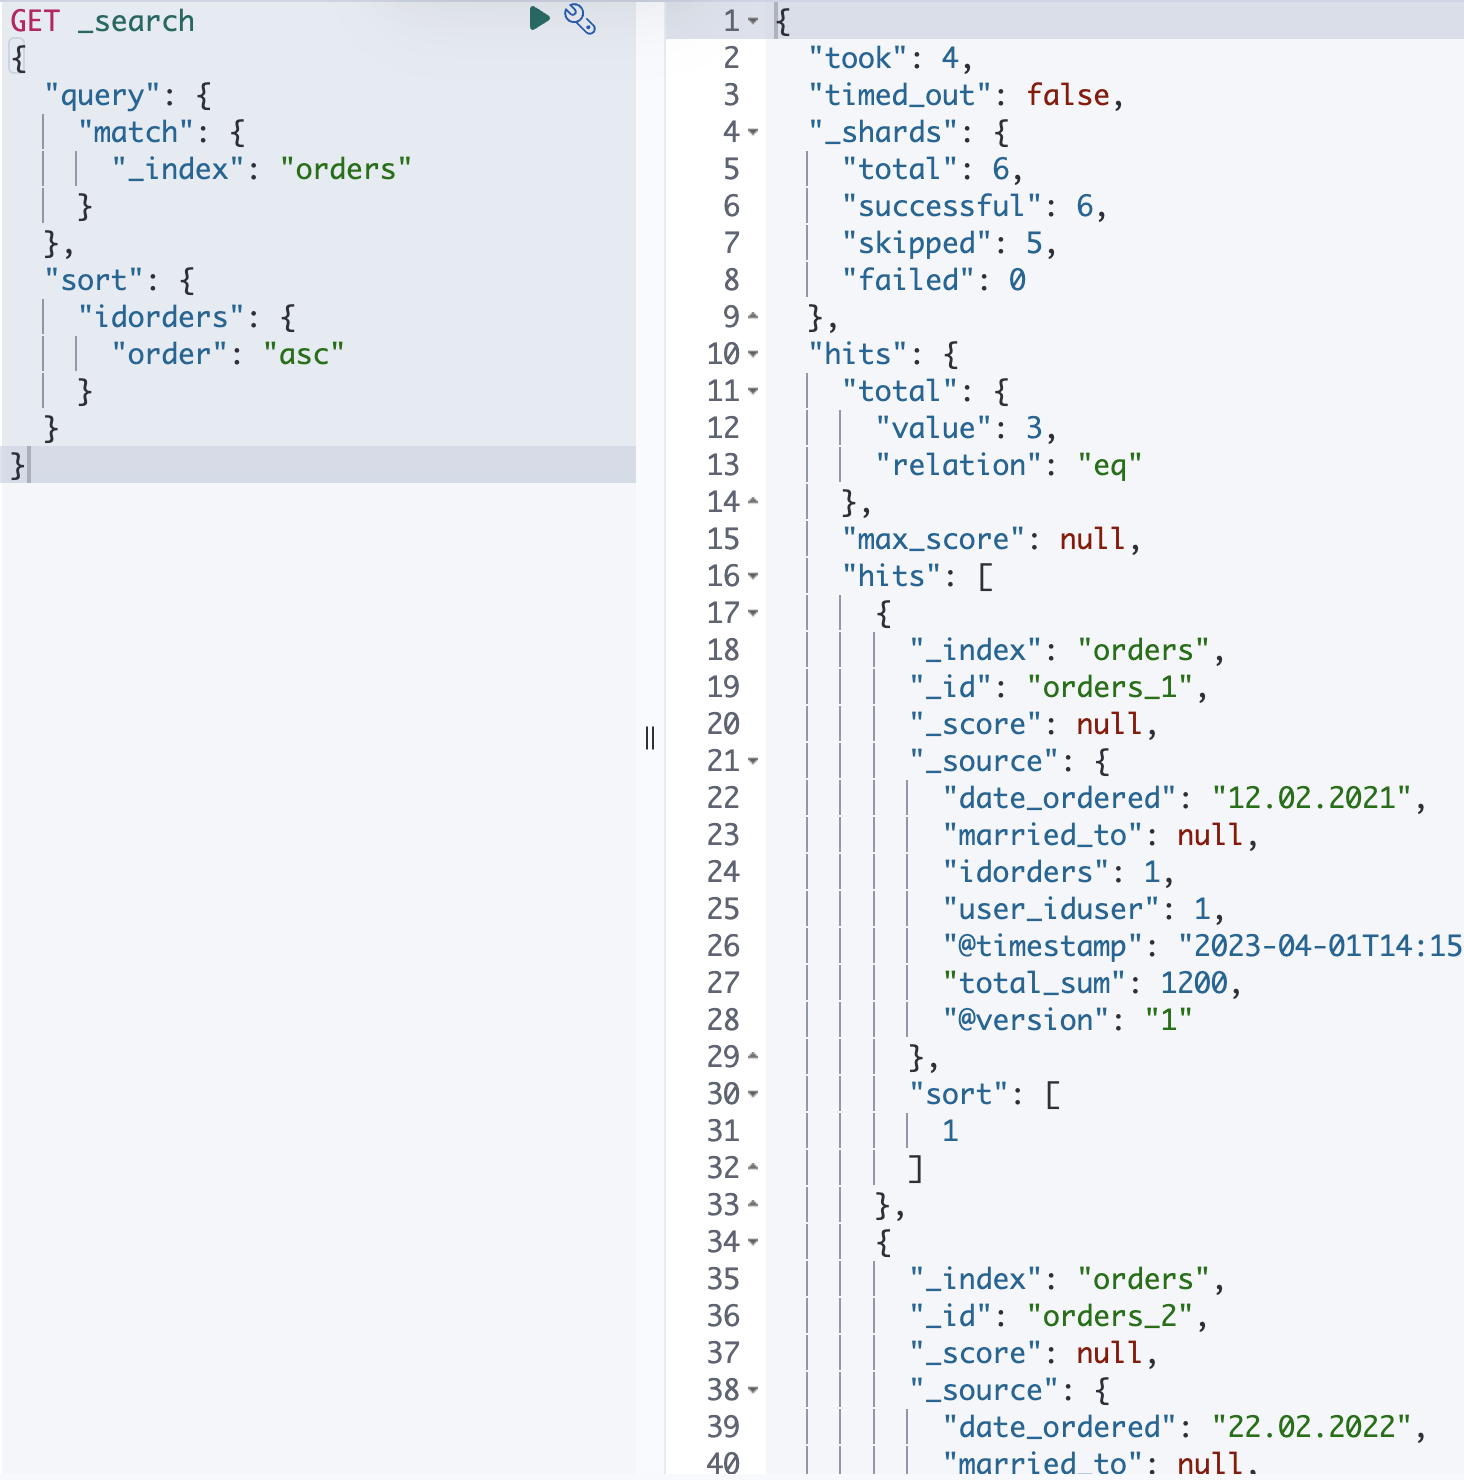
\includegraphics[height=0.45\textheight]{images/asc.png}

	\noindent \textbf{Sort desc} \\
	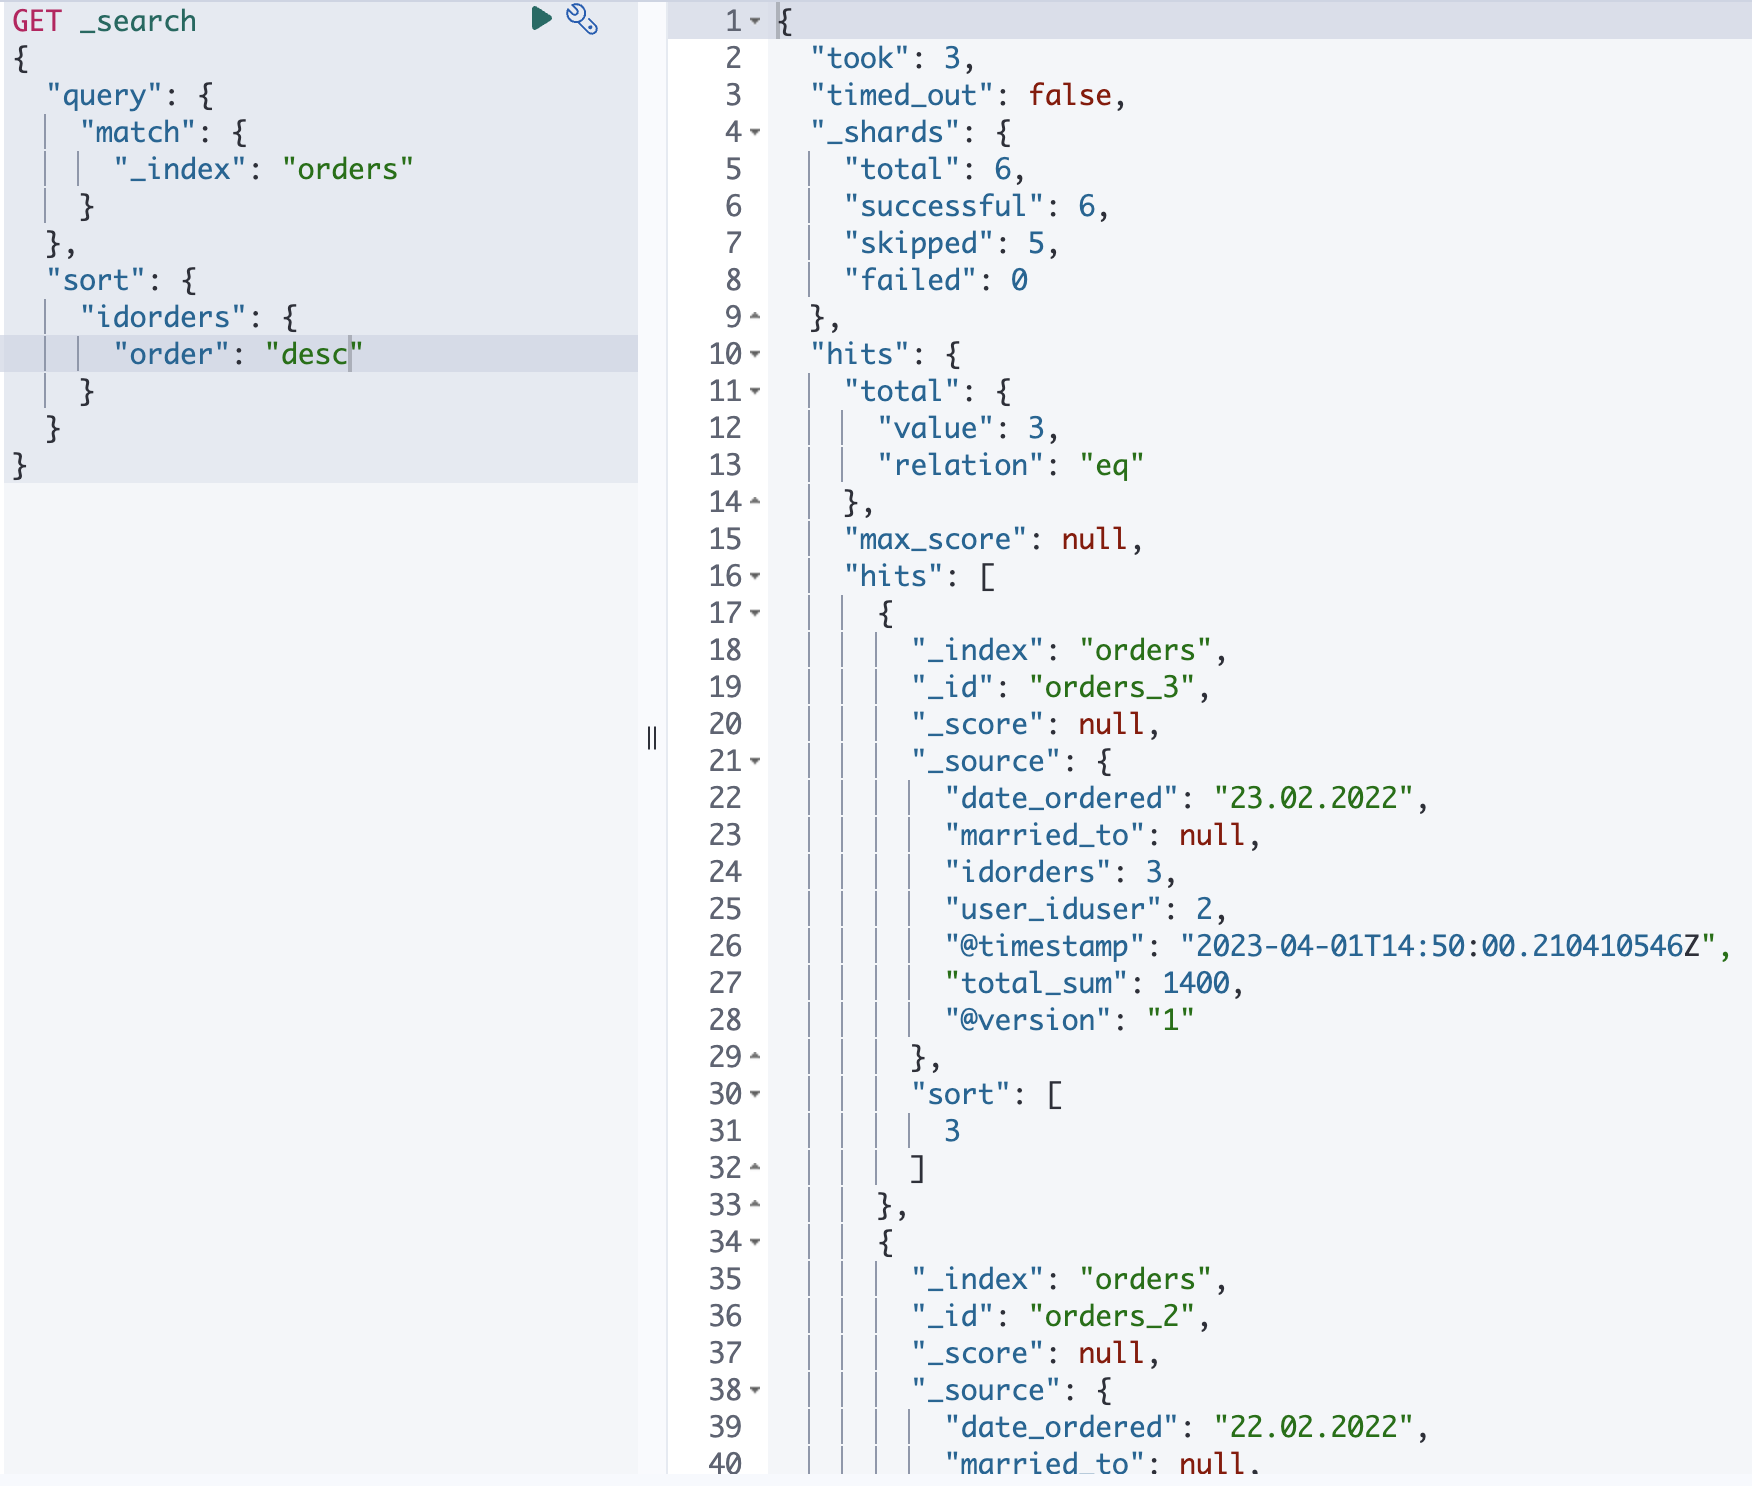
\includegraphics[height=0.45\textheight]{images/desc.png}


	\section*{Appendix}
	\subsection*{schema.sql}
	\label{listings:schema}
	\lstinputlisting[style=sql]{schema.sql}

	\subsection*{data.sql}
	\label{listings:data}
	\lstinputlisting[style=sql]{data.sql}

	\newpage

	\subsection*{logstash.conf}
	\label{listings:pipeline}
	\lstinputlisting[style=json]{logstash.conf}

	\subsection*{.env}
	\label{listings:envs}
	\lstinputlisting[style=json]{.env}
\end{document}

